% pandoc-xnos: cleveref fakery
\newcommand{\plusnamesingular}{}
\newcommand{\starnamesingular}{}
\newcommand{\xrefname}[1]{\protect\renewcommand{\plusnamesingular}{#1}}
\newcommand{\Xrefname}[1]{\protect\renewcommand{\starnamesingular}{#1}}
\providecommand{\cref}{\plusnamesingular~\ref}
\providecommand{\Cref}{\starnamesingular~\ref}
\providecommand{\crefformat}[2]{}
\providecommand{\Crefformat}[2]{}

% pandoc-xnos: cleveref formatting
\crefformat{equation}{Eq.~#2#1#3}
\Crefformat{equation}{Equation~#2#1#3}

\section{Connecting
the
dots
between
mechanosensitive
channel
abundance,
osmotic
shock,
and
survival
at
single-cell
resolution}\label{connecting-the-dots-between-mechanosensitive-channel-abundance-osmotic-shock-and-survival-at-single-cell-resolution}

Griffin
Chure\(^{a, \dagger}\),
Heun
Jin
Lee\(^{b, \dagger}\),
Akiko
Rasmussen\(^c\),
and
Rob
Phillips\(^{a,\ b,\ *}\)

\(^a\)
Department
of
Biology
and
Biological
Engineering,
California
Institute
of
Technology,
Pasadena,
CA,
USA

\(^b\)
Department
of
Physics,
California
Institute
of
Technology,
Pasadena,
California,
USA

\(^c\)
School
of
Medicine,
Medical
Sciences
and
Nutrition,
Institute
of
Medical
Sciences,
University
of
Aberdeen,
Foresterhill,
Aberdeen
AB25
2ZD
United
Kingdom

\(\dagger\)
contributed
equally

\textbf{Running
title:}
MscL
copy
number
and
cell
survival
after
osmotic
shock

* Send
correspondence
to
\texttt{phillips@pboc.caltech.edu}

\subsection{Abstract}\label{abstract}

Rapid
changes
in
extracellular
osmolarity
are
one of
many
insults
microbial
cells
face
on a
daily
basis.
To
protect
against
such
shocks,
\emph{Escherichia
coli}
and
other
microbes
express
several
types
of
transmembrane
channels
which
open
and
close
in
response
to
changes
in
membrane
tension.
In
\emph{E.
coli},
one of
the
most
abundant
channels
is the
mechanosensitive
channel
of
large
conductance
(MscL).
While
this
channel
has
been
heavily
characterized
through
structural
methods,
electrophysiology,
and
theoretical
modeling,
our
understanding
of its
physiological
role
in
preventing
cell
death
by
alleviating
high
membrane
tension
remains
tenuous.
In
this
work,
we
examine
the
contribution
of
MscL
alone
to
cell
survival
after
osmotic
shock
at
single
cell
resolution
using
quantitative
fluorescence
microscopy.
We
conduct
these
experiments
in an
\emph{E.
coli}
strain
which
is
lacking
all
mechanosensitive
channel
genes
save
for
MscL
whose
expression
is
tuned
across
three
orders
of
magnitude
through
modifications
of the
Shine-Dalgarno
sequence.
While
theoretical
models
suggest
that
only a
few
MscL
channels
would
be
needed
to
alleviate
even
large
changes
in
osmotic
pressure,
we
find
that
between
500
and
700
channels
per
cell
are
needed
to
convey
upwards
of
80\%
survival.
This
number
agrees
with
the
average
MscL
copy
number
measured
in
wild-type
\emph{E.
coli}
cells
through
proteomic
studies
and
quantitative
Western
blotting.
Furthermore,
we
observe
zero
survival
events
in
cells
with
less
than
\textasciitilde{}100
channels
per
cell.
This
work
opens
new
questions
concerning
the
contribution
of
other
mechanosensitive
channels
to
survival
as
well
as
regulation
of
their
activity.

\subsection{Importance}\label{importance}

Mechanosensitive
(MS)
channels
are
transmembrane
protein
complexes
which
open
and
close
in
response
to
changes
in
membrane
tension
as a
result
of
osmotic
shock.
Despite
extensive
biophysical
characterization,
the
contribution
of
these
channels
to
cell
survival
remains
largely
unknown.
In
this
work,
we use
quantitative
video
microscopy
to
measure
the
abundance
of a
single
species
of MS
channel
in
single
cells
followed
by
their
survival
after
a
large
osmotic
shock.
We
observe
total
death
of the
population
with
less
than
\textasciitilde{}100
channels
per
cell
and
determine
that
approximately
500 -
700
channels
are
needed
for
80\%
survival.
The
number
of
channels
we
find
to
confer
nearly
full
survival
is
consistent
with
the
counts
of the
number
of
channels
in
wild
type
cells
in
several
earlier
studies.
These
results
prompt
further
studies
to
dissect
the
contribution
of
other
channel
species
to
survival.

\subsection{Introduction}\label{introduction}

~~~~
Changes
in the
extracellular
osmolarity
can be
a
fatal
event
for
the
bacterial
cell.
Upon a
hypo-osmotic
shock,
water
rushes
into
the
cell
across
the
membrane,
leaving
the
cell
with
no
choice
but to
equalize
the
pressure.
This
equalization
occurs
either
through
damage
to the
cell
membrane
(resulting
in
death)
or
through
the
regulated
flux
of
water
molecules
through
transmembrane
protein
channels
(Fig
1A).
Such
proteinaceous
pressure
release
valves
have
been
found
across
all
domains
of
life,
with
the
first
bacterial
channel
being
described
in
1987
(\protect\hyperlink{ref-martinac1987}{1}).
Over
the
past
thirty
years,
several
more
channels
have
been
discovered,
described,
and
(in
many
cases)
biophysically
characterized.
\emph{E.
coli},
for
example,
has
seven
of
these
channels
(one
MscL
and
six
MscS
homologs)
which
have
varied
conductance,
gating
mechanisms,
and
expression
levels.
While
they
have
been
the
subject
of
much
experimental
and
theoretical
dissection,
much
remains
a
mystery
with
regard
to the
roles
their
abundance
and
interaction
with
other
cellular
processes
play
in the
greater
context
of
physiology
(\protect\hyperlink{ref-bavi2016}{2}--\protect\hyperlink{ref-vandenberg2016}{8}).

~~ ~
~Of
the
seven
channels
in
\emph{E.
coli},
the
mechanosensitive
channel
of
large
conductance
(MscL)
is one
of the
most
abundant
and
the
best
characterized.
This
channel
has a
large
conductance
(3 nS)
and
mediates
the
flux
of
water
molecules
across
the
membrane
via a
\textasciitilde{}3
nm
wide
pore
in the
open
state
(\protect\hyperlink{ref-cruickshank1997}{9},
\protect\hyperlink{ref-haswell2011}{10}).
Molecular
dynamics
simulations
indicate
that a
single
open
MscL
channel
permits
the
flux
of
\(4 \times 10^9\)
water
molecules
per
second,
which
is an
order
of
magnitude
larger
than a
single
aquaporin
channel
(BNID
100479)
(\protect\hyperlink{ref-louhivuori2010}{11},
\protect\hyperlink{ref-milo2010}{12}).
This
suggests
that
having
only a
few
channels
per
cell
could
be
sufficient
to
relieve
even
large
changes
in
membrane
tension.
Electrophysiological
experiments
have
suggested
a
small
number
of
channels
per
cell
(\protect\hyperlink{ref-booth2005}{13},
\protect\hyperlink{ref-hase1997}{14}),
however,
more
recent
approaches
using
quantitative
Western
blotting,
fluorescence
microscopy,
and
proteomics
have
measured
several
hundred
MscL
per
cell
(\protect\hyperlink{ref-bialecka-fornal2012}{3},
\protect\hyperlink{ref-schmidt2016}{15},
\protect\hyperlink{ref-soufi2015}{16}).
To
further
complicate
matters,
the
expression
profile
of
MscL
appears
to
depend
on
growth
phase,
available
carbon
source,
and
other
environmental
challenges
(\protect\hyperlink{ref-bialecka-fornal2012}{3},
\protect\hyperlink{ref-soufi2015}{16},
\protect\hyperlink{ref-stokes2003a}{17}).
While
there
are
likely
more
than
just a
few
channels
per
cell,
why
cells
seem
to
need
so
many
and
the
biological
rationale
behind
their
condition-dependent
expression
both
remain
a
mystery.

~~~ ~
While
their
biochemical
and
biophysical
characteristics
have
received
much
attention,
their
connection
to
cell
survival
is
understudied.
Drawing
such a
direct
connection
between
channel
copy
number
and
survival
requires
quantitative
\emph{in
vivo}
experiments.
To our
knowledge,
the
work
presented
in van
den
Berg
et al.
2016
(\protect\hyperlink{ref-vandenberg2016}{8})
is the
first
attempt
to
simultaneously
measure
channel
abundance
and
survivability
for a
single
species
of
mechanosensitive
channel.
While
the
measurement
of
channel
copy
number
was
performed
at the
level
of
single
cells
using
super-resolution
microscopy,
survivability
after
a
hypo-osmotic
shock
was
assessed
in
bulk
plating
assays
which
rely
on
serial
dilutions
of a
shocked
culture
followed
by
counting
the
number
of
resulting
colonies
after
incubation.
Such
bulk
assays
have
long
been
the
standard
for
querying
cell
viability
after
an
osmotic
challenge.
While
they
have
been
highly
informative,
they
reflect
only
the
mean
survival
rate
of the
population,
obfuscating
the
variability
in
survival
of the
population.
The
stochastic
nature
of
gene
expression
results
in a
noisy
distribution
of
MscL
channels
rather
than a
single
value,
meaning
those
found
in the
long
tails
of the
distribution
have
quite
different
survival
rates
than
the
mean
but
are
lost
in the
final
calculation
of
survival
probability.

~ ~ ~
~In
this
work,
we
present
an
experimental
system
to
quantitatively
probe
the
interplay
between
MscL
copy
number
and
survival
at
single-cell
resolution,
as is
seen
in
Fig.~\ref{fig:overview}B.
We
generated
an
\emph{E.
coli}
strain
in
which
all
seven
mechanosensitive
channels
had
been
deleted
from
the
chromosome
followed
by a
chromosomal
integration
of a
single
gene
encoding
an
MscL-super-folder
GFP
(sfGFP)
fusion
protein.
To
explore
copy
number
regimes
beyond
those
of the
wild-type
expression
level,
we
modified
the
Shine-Dalgarno
sequence
of
this
integrated
construct,
allowing
us to
cover
nearly
three
decades
of
MscL
copy
number.
To
probe
survivability,
we
exposed
cells
to a
large
hypo-osmotic
shock
at
controlled
rates
in a
flow
cell
under
a
microscope,
allowing
the
observation
of the
single-cell
channel
copy
number
and
the
resulting
survivability
of
single
cells.
With
this
large
set of
single
cell
measurements,
we
approach
the
calculation
of
survival
probability
in a
manner
that
is
free
of
binning
bias
which
allows
the
reasonable
extrapolation
of
survival
probability
to
copy
numbers
outside
of the
observed
range.
In
addition,
we
show
that
several
hundred
channels
are
needed
to
convey
high
rates
of
survival
and
observe
a
minimum
number
of
channels
needed
to
permit
any
degree
of
survival.

\begin{figure}
\centering
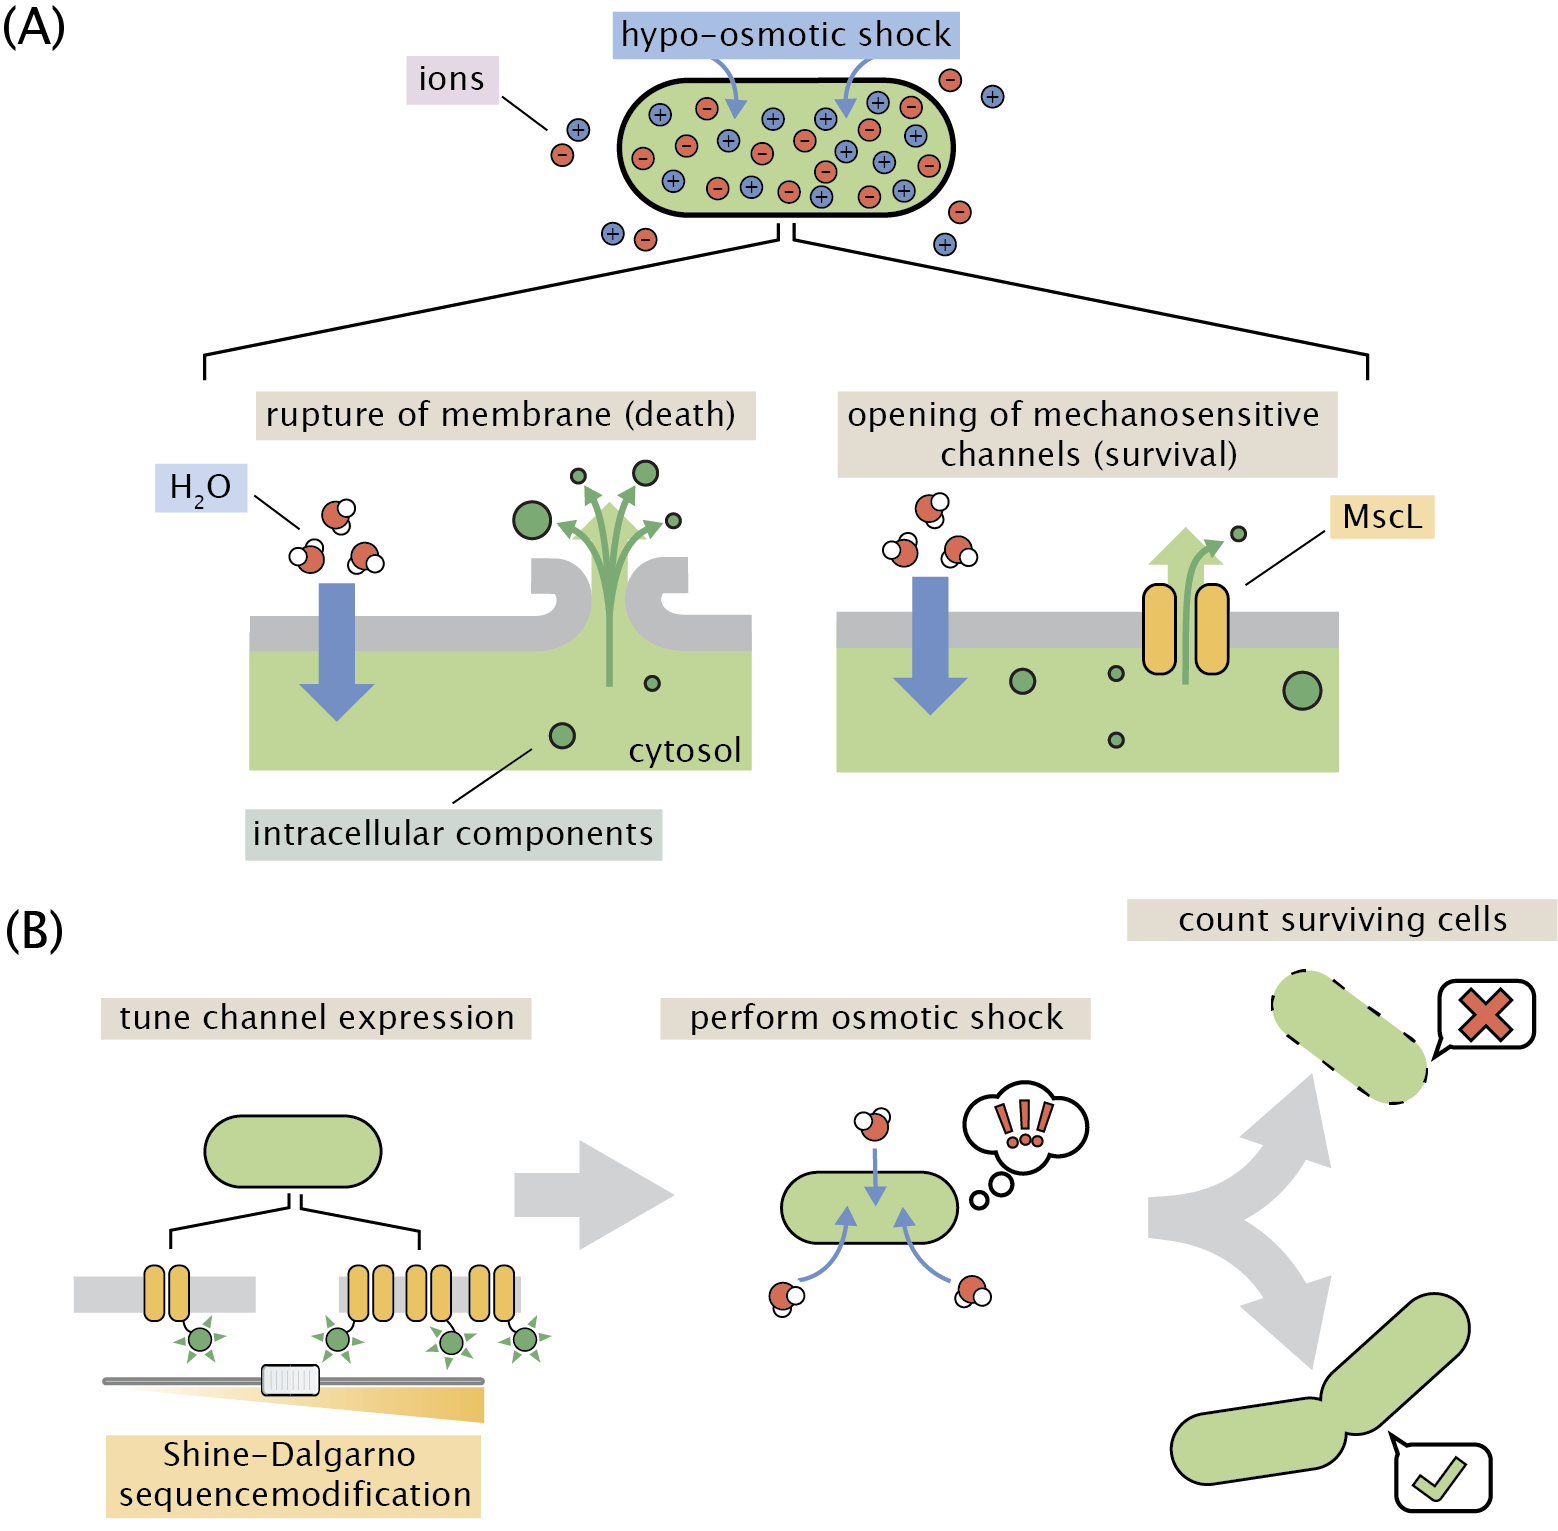
\includegraphics{../figs/fig1.pdf}
\caption{Role
of
mechanosensitive
channels
during
hypo-osmotic
shock.
(A) A
hypo-osmotic
shock
results
in a
large
difference
in the
osmotic
strength
between
the
intracellular
and
extracellular
spaces.
As a
result,
water
rushes
into
the
cell
to
equalize
this
gradient
increasing
the
turgor
pressure
and
tension
in the
cell
membrane.
If no
mechanosensitive
channels
are
present
and
membrane
tension
is
high
(left
panel),
the
membrane
ruptures
releasing
intracellular
content
into
the
environment
resulting
in
cell
death
. If
mechanosensitive
channels
are
present
(right
panel)
and
membrane
tension
is
beyond
the
gating
tension,
the
mechanosensitive
channel
MscL
opens,
releasing
water
and
small
intracellular
molecules
into
the
environment
thus
relieving
pressure
and
membrane
tension.
(B)
The
experimental
approach
undertaken
in
this
work.
The
number
of
mechanosensitive
channels
tagged
with a
fluorescent
reporter
is
tuned
through
modification
of the
Shine-Dalgarno
sequence
of the
\emph{mscL}
gene.
The
cells
are
then
subjected
to a
hypo-osmotic
shock
and
the
number
of
surviving
cells
are
counted,
allowing
the
calculation
of a
survival
probability.}\label{fig:overview}
\end{figure}

\subsection{Results}\label{results}

\subsubsection{Quantifying
the
single-cell
MscL
copy
number}\label{quantifying-the-single-cell-mscl-copy-number}

~~~~The
principal
goal
of
this
work
is to
examine
the
contribution
of a
single
mechanosensitive
channel
species
to
cell
survival
under
a
hypo-osmotic
shock.
While
this
procedure
could
be
performed
for
any
species
of
channel,
we
chose
MscL
as it
is the
most
well
characterized
and
one of
the
most
abundant
species
in
\emph{E.
coli}.
To
probe
the
contribution
of
MscL
alone,
we
integrated
an
\emph{mscL}
gene
encoding
an
MscL
super-folder
GFP
(sfGFP)
fusion
into a
strain
in
which
all
seven
known
mechanosensitive
channel
genes
were
deleted
from
the
chromosome
(\protect\hyperlink{ref-edwards2012}{5}).
Chromosomal
integration
imposes
strict
control
on the
gene
copy
number
compared
to
plasmid
borne
expression
systems,
which
is
important
to
minimize
variation
in
channel
expression
across
the
population
and
provide
conditions
more
representative
of
native
cell
physiology.
Abrogation
of
activity,
mislocalization,
or
cytotoxicity
are
all
inherent
risks
associated
with
creating
chimeric
reporter
constructs.
In
Supplement
A, we
carefully
dissect
the
functionality
of
this
protein
through
electrophysiology
(Fig.
S1),
measure
the
rate
of
fluorophore
maturation
(Fig.
S2),
and
quantify
potential
aggregates
(Figs.
S3 and
S4).
To the
best
of our
knowledge,
the
MscL-sfGFP
fusion
protein
functions
identically
to the
wild-type,
allowing
us to
confidently
draw
conclusions
about
the
physiological
role
this
channel
plays
in
wild-type
cells.

~~~~To
modulate
the
number
of
MscL
channels
per
cell,
we
developed
a
series
of
mutants
which
were
designed
to
decrease
the
expression
relative
to
wild-type.
These
changes
involved
direct
alterations
of the
Shine-Dalgarno
sequence
as
well
as the
inclusion
of AT
hairpins
of
varying
length
directly
upstream
of the
start
codon
which
influences
the
translation
rate
and
hence
the
number
of
MscL
proteins
produced
(Fig.~\ref{fig:boxplot}A).
The
six
Shine-Dalgarno
sequences
used
in
this
work
were
chosen
using
the
RBS
binding
site
strength
calculator
from
the
Salis
Laboratory
at the
Pennsylvania
State
University
(\protect\hyperlink{ref-espahborujeni2014}{18},
\protect\hyperlink{ref-salis2009}{19}).
While
the
designed
Shine-Dalgarno
sequence
mutations
decreased
the
expression
relative
to
wild-type
as
intended,
the
distribution
of
expression
is
remarkably
wide
spanning
an
order
of
magnitude.

~~~~To
measure
the
number
of
MscL
channels
per
cell,
we
determined
a
fluorescence
calibration
factor
to
translate
arbitrary
fluorescence
units
per
cell
to
protein
copy
number.
While
there
have
been
numerous
techniques
developed
over
the
past
decade
to
directly
measure
this
calibration
factor,
such
as
quantifying
single-molecule
photobleaching
constants
or
measuring
the
binomial
partitioning
of
fluorescent
proteins
upon
cell
division
(\protect\hyperlink{ref-bialecka-fornal2012}{3},
\protect\hyperlink{ref-elowitz2002}{20}),
we
used
\emph{a
priori}
knowledge
of the
mean
MscL-sfGFP
expression
level
of a
particular
\emph{E.
coli}
strain
to
estimate
the
average
fluorescence
of a
single
channel.
In
Bialecka-Fornal
et al.
2012
(\protect\hyperlink{ref-bialecka-fornal2012}{3}),
the
authors
used
single-molecule
photobleaching
and
quantitative
Western
blotting
to
probe
the
expression
of
MscL-sfGFP
under
a wide
range
of
growth
conditions.
To
compute
a
calibration
factor,
we
used
the
strain
MLG910
(\emph{E.
coli}
K12
MG1655
\(\phi\)(mscL-sfGFP))
as a
``standard
candle'',
highlighted
in
yellow
in
Fig.~\ref{fig:boxplot}B.
This
standard
candle
strain
was
grown
and
imaged
in
identical
conditions
in
which
the
MscL
count
was
determined
through
fluorescence
microscopy.
The
calibration
factor
was
computed
by
dividing
the
mean
total
cell
fluorescence
by the
known
MscL
copy
number,
resulting
in a
measure
of
arbitrary
fluorescence
units
per
MscL
channel.
Details
regarding
this
calculation
and
appropriate
propagation
of
error
as
well
as its
sensitivity
to
varying
growth
media
can be
found
in the
Materials
\&
Methods
as
well
as
Supplement
B
(Fig.
S5 -
S8).

~~~~While
it is
seemingly
straightforward
to use
this
calibration
factor
to
determine
the
total
number
of
channels
per
cell
for
wild-type
or
highly
expressing
strains,
the
calculation
for
the
lowest
expressing
strains
is
complicated
by
distorted
cell
morphology.
We
observed
that
as the
channel
copy
number
decreases,
cellular
morphology
becomes
increasingly
aberrant
with
filamentous,
bulging,
and
branched
cells
becoming
more
abundant
(Fig.
S7A).
This
morphological
defect
has
been
observed
when
altering
the
abundance
of
several
species
of
mechanosensitive
channels,
suggesting
that
they
play
an
important
role
in
general
architectural
stability
(\protect\hyperlink{ref-bialecka-fornal2012}{3},
\protect\hyperlink{ref-bialecka-fornal2015}{4}).
As
these
aberrant
morphologies
can
vary
widely
in
size
and
shape,
calculating
the
number
of
channels
per
cell
becomes
a more
nuanced
endeavor.
For
example,
taking
the
total
MscL
copy
number
for
these
cells
could
skew
the
final
calculation
of
survival
probability
as a
large
but
severely
distorted
cell
would
be
interpreted
as
having
more
channels
than a
smaller,
wild-type
shaped
cell
(Fig.
S7B).
To
correct
for
this
pathology,
we
computed
the
average
expression
level
per
unit
area
for
each
cell
and
multiplied
this
by the
average
cellular
area
of our
standard
candle
strain
which
is
morphologically
indistinguishable
from
wild-type
\emph{E.
coli},
allowing
for
the
calculation
of an
effective
channel
copy
number.
The
effect
of
this
correction
can be
seen
in
Fig.
S7C
and D,
which
illustrate
that
there
is no
other
correlation
between
cell
area
and
channel
expression.

~~~~Our
calculation
of the
effective
channel
copy
number
for
our
suite
of
Shine-Dalgarno
mutants
is
shown
in
Fig.~\ref{fig:boxplot}B.
The
expression
of
these
strains
cover
nearly
three
orders
of
magnitude
with
the
extremes
ranging
from
approximately
four
channels
per
cell
to
nearly
one
thousand.
While
the
means
of
each
strain
are
somewhat
distinct,
the
distributions
show a
large
degree
of
overlap,
making
one
strain
nearly
indistinguishable
from
another.
This
variance
is a
quantity
that
is
lost
in the
context
of
bulk
scale
experiments
but
can be
accounted
for
via
single-cell
methods.

\begin{figure}
\centering
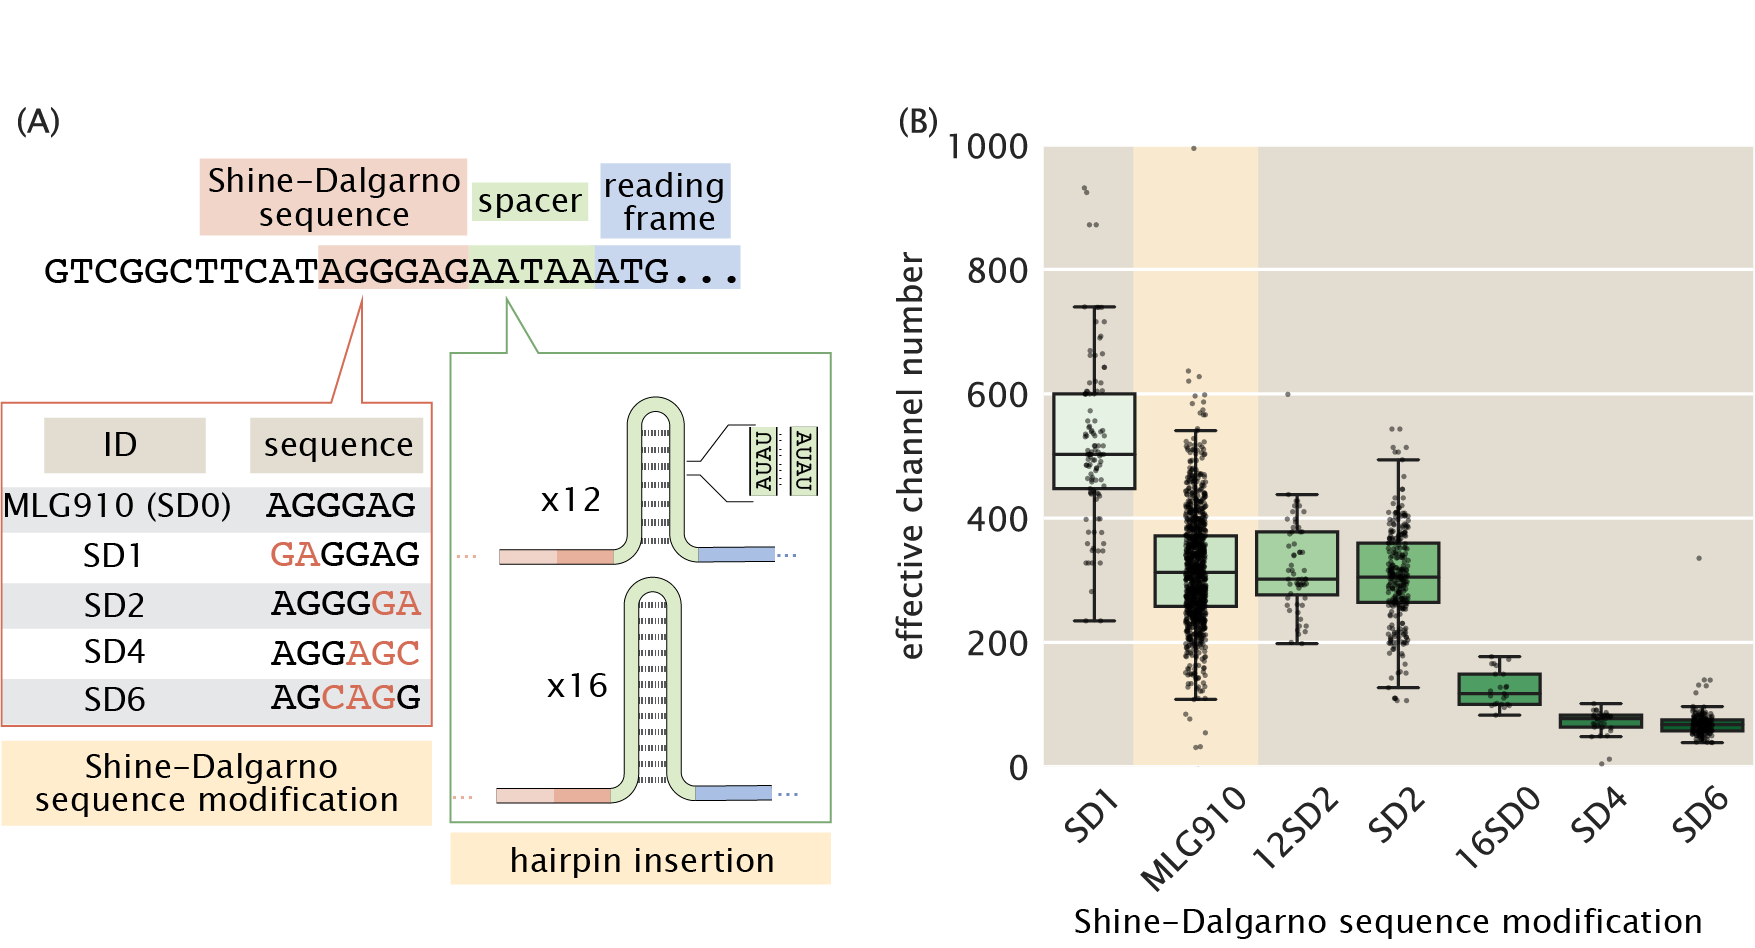
\includegraphics{../figs/fig2.pdf}
\caption{Control
of
MscL
expression
and
calculation
of
channel
copy
number.
(A)
Schematic
view
of the
expression
modifications
performed
in
this
work.
The
beginning
portion
of the
native
\emph{mscL}
sequence
is
shown
with
the
Shine-Dalgarno
sequence,
spacer
region,
and
start
codon
shaded
in
red,
green,
and
blue,
respectively.
The
Shine-Dalgarno
sequence
was
modified
through
the
Salis
lab
Ribosomal
Binding
Strength
calculator
(\protect\hyperlink{ref-espahborujeni2014}{18},
\protect\hyperlink{ref-salis2009}{19}).
The
wild-type
sequence
(MLG910)
is
shown
in
black
with
mutations
for
the
other
four
Shine-Dalgarno
mutants
highlighted
in
red.
Expression
was
further
modified
by the
insertion
of
repetitive
\texttt{AT}
bases
into
the
spacer
region,
generating
hairpins
of
varying
length
which
acted
as a
thermodynamic
barrier
for
translation
initiation.
(B)
Variability
in
effective
channel
copy
number
is
computed
using
the
standard
candle.
The
boxes
represent
the
interquartile
region
of the
distribution,
the
center
line
displays
the
median,
and
the
whiskers
represent
1.5
times
the
maximum
and
minimum
of the
interquartile
region.
Individual
measurements
are
denoted
as
black
points.
The
strain
used
for
calibration
of
channel
copy
number
(MLG910)
is
highlighted
in
yellow.}\label{fig:boxplot}
\end{figure}

\subsubsection{Performing
a
single-cell
hypo-osmotic
challenge
assay}\label{performing-a-single-cell-hypo-osmotic-challenge-assay}

~~~~To
measure
the
channel
copy
number
of a
single
cell
and
query
its
survival
after
a
hypo-osmotic
shock,
we
used a
custom-made
flow
cell
in
which
osmotic
shock
and
growth
can be
monitored
in
real
time
using
video
microscopy
(Fig.~\ref{fig:flow_cell}A).
The
design
and
characterization
of
this
device
has
been
described
in
depth
previously
and is
briefly
described
in the
Materials
\&
Methods
(\protect\hyperlink{ref-bialecka-fornal2015}{4}).
Using
this
device,
cells
were
exposed
to a
large
hypo-osmotic
shock
by
switching
between
LB
Lennox
medium
supplemented
with
500 mM
NaCl
and LB
Lennox
media
alone.
All
six
Shine-Dalgarno
modifications
shown
in
Fig.~\ref{fig:boxplot}B
(excluding
MLG910)
were
subjected
to a
hypo-osmotic
shock
at
controlled
rates
while
under
observation.
After
the
application
of the
osmotic
shock,
the
cells
were
imaged
every
sixty
seconds
for
four
to six
hours.
Each
cell
was
monitored
over
the
outgrowth
period
and
was
manually
scored
as
either
a
survivor,
fatality,
or
inconclusive
observation.
The
criteria
used
for
scoring
death
were
the
same
as
those
previously
described
in
Bialecka-Fornal
et al.
2015
(\protect\hyperlink{ref-bialecka-fornal2015}{4}).
Survivors
were
defined
as
cells
that
underwent
multiple
divisions
post-shock.
To
qualify
as
survivors,
cells
must
undergo
at
least
two
divisions,
although
more
typically,
four
to
eight
divisions
are
observed
without
any
signs
of
slowing
down.
Imaging
is
stopped
when
the
survivors
cells
begin
to go
out of
focus
or
overlap
each
other.
Survivors
do not
show
any
sign
of
ceasing
division.
More
information
regarding
this
classification
can be
found
in the
Materials
and
Methods
as
well
as
Supplement
C
(Fig.
S9 -
S10
and
Table
S1 -
S2).
The
brief
experimental
protocol
can be
seen
in
Fig.~\ref{fig:flow_cell}B.

\begin{figure}
\centering
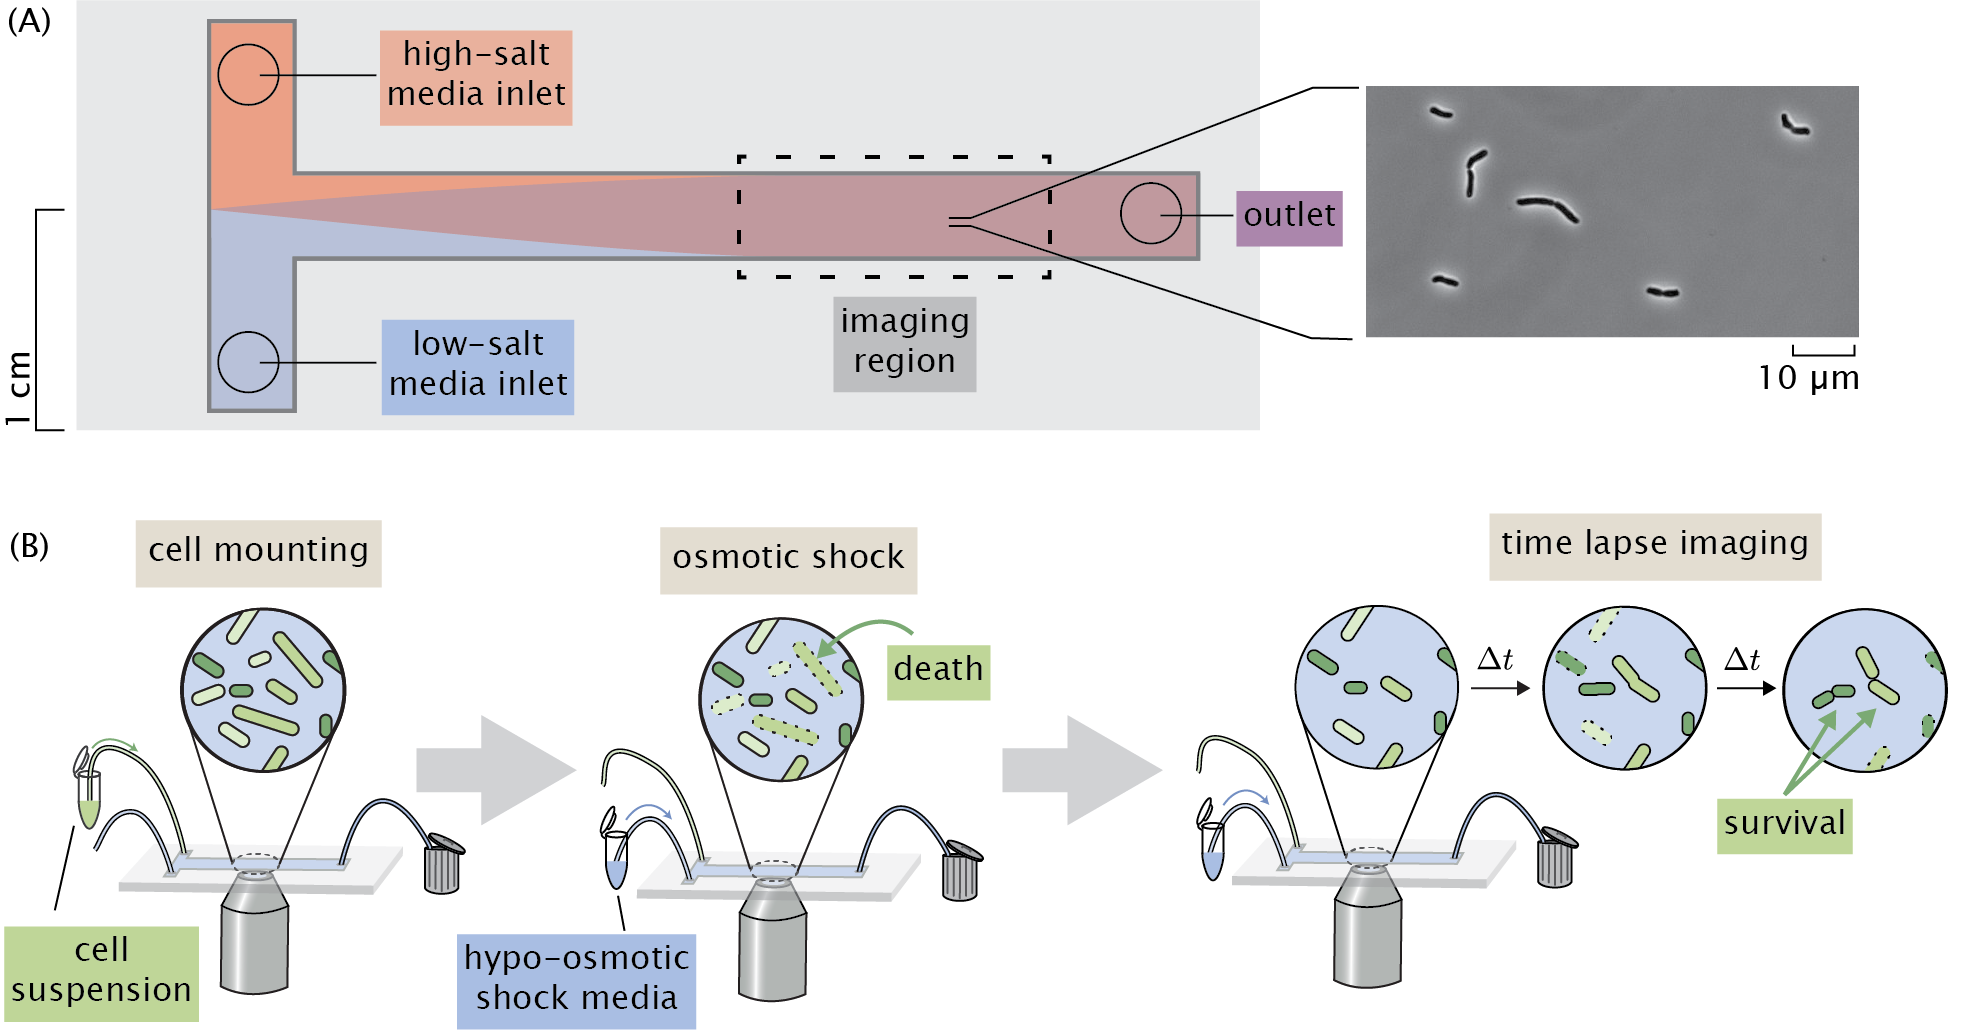
\includegraphics{../figs/fig3.pdf}
\caption{Experimental
approach
to
measuring
survival
probability.
(A)
Layout
of a
home-made
flow
cell
for
subjecting
cells
to
osmotic
shock.
Cells
are
attached
to a
polyethylenimine
functionalized
surface
of a
glass
coverslip
within
the
flow
chamber
by
loading
a
dilute
cell
suspension
through
one of
the
inlets.
(B)
The
typical
experimental
procedure.
Cells
are
loaded
into a
flow
chamber
as
shown
in (A)
and
mounted
to the
glass
coverslip
surface.
Cells
are
subjected
to a
hypo-osmotic
shock
by
flowing
hypotonic
medium
into
the
flow
cell.
After
shock,
the
cells
are
monitored
for
several
hours
and
surviving
cells
are
identified.}\label{fig:flow_cell}
\end{figure}

~~~~Due
to the
extensive
overlap
in
expression
between
the
different
Shine-Dalgarno
mutants
(see
Fig.~\ref{fig:boxplot}B),
computing
the
survival
probability
by
treating
each
mutant
as an
individual
bin
obfuscates
the
relationship
between
channel
abundance
and
survival.
To
more
thoroughly
examine
this
relationship,
all
measurements
were
pooled
together
with
each
cell
being
treated
as an
individual
experiment.
The
hypo-osmotic
shock
applied
in
these
experiments
was
varied
across
a
range
of
0.02
Hz
(complete
exchange
in 50
s) to
2.2 Hz
(complete
exchange
in
0.45
s).
Rather
than
pooling
this
wide
range
of
shock
rates
into a
single
data
set,
we
chose
to
separate
the
data
into
``slow
shock''
(
\textless{}
1.0
Hz)
and
``fast
shock''
(\(\geq 1.0\)
Hz)
classes.
Other
groupings
of
shock
rate
were
explored
and
are
discussed
in
Supplement
D
(Fig.
S11
and
S12).
The
cumulative
distributions
of
channel
copy
number
separated
by
survival
are
shown
in
Fig.~\ref{fig:survival_dists}.
In
these
experiments,
survival
was
never
observed
for a
cell
containing
less
than
approximately
100
channels
per
cell,
indicated
by the
red
stripe
in
Fig.~\ref{fig:survival_dists}.
This
suggests
that
there
is a
minimum
number
of
channels
needed
for
survival
on the
order
of 100
per
cell.
We
also
observe
a
slight
shift
in the
surviving
fraction
of the
cells
towards
higher
effective
copy
number,
which
matches
our
intuition
that
including
more
mechanosensitive
channels
increases
the
survival
probability.

\begin{figure}
\centering
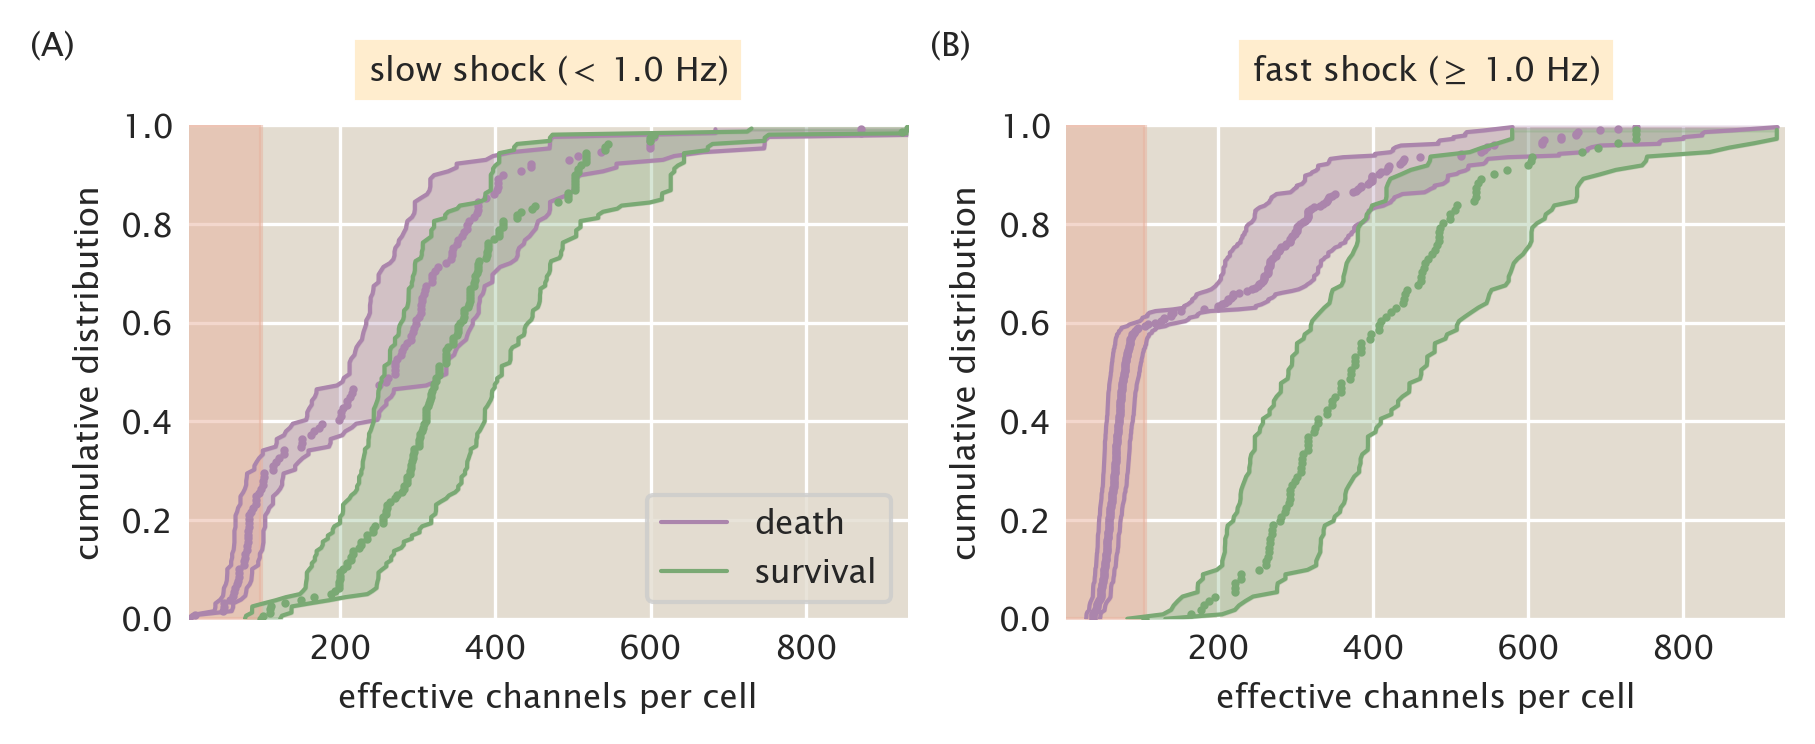
\includegraphics{../figs/fig4.pdf}
\caption{Distributions
of
survival
and
death
as a
function
of
effective
channel
number.
(A)
Empirical
cumulative
distributions
of
channel
copy
number
separated
by
survival
(green)
or
death
(purple)
after
a slow
(\(< 1.0\)
Hz)
osmotic
shock.
(B)
The
empirical
cumulative
distribution
for a
fast
(\(\geq 1.0\)
Hz)
osmotic
shock.
Shaded
green
and
purple
regions
represent
the
95\%
credible
region
of the
effective
channel
number
calculation
for
each
cell.
Shaded
red
stripe
signifies
the
range
of
channels
in
which
no
survival
was
observed.}\label{fig:survival_dists}
\end{figure}

\subsubsection{Prediction
of
survival
probability
as a
function
of
channel
copy
number}\label{prediction-of-survival-probability-as-a-function-of-channel-copy-number}

~~~~There
are
several
ways
by
which
the
survival
probability
can be
calculated.
The
most
obvious
approach
would
be to
group
each
individual
Shine-Dalgarno
mutant
as a
single
bin
and
compute
the
average
MscL
copy
number
and
the
survival
probability.
Binning
by
strain
is the
most
frequently
used
approach
for
such
measurements
and
has
provided
valuable
insight
into
the
qualitative
relationship
of
survival
on
other
physiological
factors
(\protect\hyperlink{ref-bialecka-fornal2015}{4},
\protect\hyperlink{ref-vandenberg2016}{8}).
However
the
copy
number
distribution
for
each
Shine-Dalgarno
mutant
(Fig.~\ref{fig:boxplot}B)
is
remarkably
wide
and
overlaps
with
the
other
strains.
We
argue
that
this
coarse-grained
binning
negates
the
benefits
of
performing
single-cell
measurements
as two
strains
with
different
means
but
overlapping
quartiles
would
be
treated
as
distinctly
different
distributions.

~~~~Another
approach
would
be to
pool
all
data
together,
irrespective
of the
Shine-Dalgarno
mutation,
and
bin by
a
defined
range
of
channels.
Depending
on the
width
of the
bin,
this
could
allow
for
finer
resolution
of the
quantitative
trend,
but
the
choice
of the
bin
width
is
arbitrary
with
the
\emph{a
priori}
knowledge
that
is
available.
Drawing
a
narrow
bin
width
can
easily
restrict
the
number
of
observed
events
to
small
numbers
where
the
statistical
precision
of the
survival
probability
is
lost.
On the
other
hand,
drawing
wide
bins
increases
the
precision
of the
estimate,
but
becomes
further
removed
from a
true
single-cell
measurement
and
represents
a
population
mean,
even
though
it may
be a
smaller
population
than
binning
by the
Shine-Dalgarno
sequence
alone.
In
both
of
these
approaches,
it is
difficult
to
extrapolate
the
quantitative
trend
outside
of the
experimentally
observed
region
of
channel
copy
number.
Here,
we
present
a
method
to
estimate
the
probability
of
survival
for
any
channel
copy
number,
even
those
that
lie
outside
of the
experimentally
queried
range.

~~~~To
quantify
the
survival
probability
while
maintaining
single-cell
resolution,
we
chose
to use
a
logistic
regression
model
which
does
not
require
grouping
data
into
arbitrary
bins
and
treats
each
cell
measurement
as an
independent
experiment.
Logistic
regression
is an
inferential
method
to
model
the
probability
of a
Boolean
or
categorical
event
(such
as
survival
or
death)
given
one or
several
predictor
variables
and is
commonly
used
in
medical
statistics
to
compute
survival
rates
and
dose
response
curves
(\protect\hyperlink{ref-anderson2003}{21},
\protect\hyperlink{ref-mishra2016}{22}).
The
primary
assumption
of
logistic
regression
is
that
the
log-odds
probability
of
survival
\(p_{s}\)
is
linearly
dependent
on the
predictor
variable,
in our
case
the
log
channels
per
cell
\(N_{c}\)
with a
dimensionless
intercept
\(\beta_0\)
and
slope
\(\beta_1\),
\begin{equation}
\log{p_s \over 1 - p_s} = \beta_0 + \beta_1 \log N_c.
\label{eq:linear_channel_logit}\end{equation}
Under
this
assumption
of
linearity,
\(\beta_0\)
is the
log-odds
probability
of
survival
with
no
MscL
channels.
The
slope
\(\beta_1\)
represents
the
change
in the
log-odds
probability
of
survival
conveyed
by a
single
channel.
As the
calculated
number
of
channels
in
this
work
spans
nearly
three
orders
of
magnitude,
it is
better
to
perform
this
regression
on
\(\log N_c\)
as
regressing
on
\(N_c\)
directly
would
give
undue
weight
for
lower
channel
copy
numbers
due to
the
sparse
sampling
of
high-copy
number
cells.
The
functional
form
shown
in
Eq.~\ref{eq:linear_channel_logit}
can be
derived
directly
from
Bayes'
theorem
and is
shown
in
Supplement
E. If
one
knows
the
values
of
\(\beta_0\)
and
\(\beta_1\),
the
survival
probability
can be
expressed
as
\begin{equation}
p_s = \frac{1}{1 + N_c^{-\beta_1}e^{-\beta_0}}.
\label{eq:prob}\end{equation}
In
this
analysis,
we
used
Bayesian
inferential
methods
to
determine
the
most
likely
values
of the
coefficients
and is
described
in
detail
in the
Supplement
E
(Fig.
S13
and
S14).

~~~~
The
results
of the
logistic
regression
are
shown
in
Fig.~\ref{fig:survival}.
We see
a
slight
rightward
shift
the
survival
probability
curve
under
fast
shock
relative
to the
slow
shock
case,
reaffirming
the
conclusion
that
survival
is
also
dependent
on the
rate
of
osmotic
shock
(\protect\hyperlink{ref-bialecka-fornal2015}{4}).
This
rate
dependence
has
been
observed
for
cells
expressing
MscL
alongside
other
species
of
mechanosensitive
channels,
but
not
for
MscL
alone.
This
suggests
that
MscL
responds
differently
to
different
rates
of
shock,
highlighting
the
need
for
further
study
of
rate
dependence
and
the
coordination
between
different
species
of
mechanosensitive
channels.
Fig.~\ref{fig:survival}
also
shows
that
several
hundred
channels
are
required
to
provide
appreciable
protection
from
osmotic
shock.
For a
survival
probability
of
80\%,
a cell
must
have
approximately
500 to
700
channels
per
cell
for a
fast
and
slow
shock,
respectively.
The
results
from
the
logistic
regression
are
showed
as
continuous
colored
curves.
The
individual
cell
measurements
separated
by
survival
and
death
are
shown
at the
top
and
bottom
of
each
plot,
respectively,
and
are
included
to
provide
a
sense
of
sampling
density.

~~~~Over
the
explored
range
of
MscL
copy
number,
we
observed
a
maximum
of
80\%
survival
for
any
binning
method.
The
remaining
20\%
survival
may be
attained
when
the
other
species
of
mechanosensitive
channels
are
expressed
alongside
MscL.
However,
it is
possible
that
the
flow
cell
method
performed
in
this
work
lowers
the
maximal
survival
fraction
as the
cells
are
exposed
to
several,
albeit
minor,
mechanical
stresses
such
as
loading
into
the
flow
cell
and
chemical
adherence
to the
glass
surface.
To
ensure
that
the
results
from
logistic
regression
accurately
describe
the
data,
we can
compare
the
survival
probabilities
to
those
using
the
binning
methods
described
earlier
(red
and
black
points,
Fig.~\ref{fig:survival}).
Nearly
all
binned
data
fall
within
error
of the
prediction
(see
Materials
\&
Methods
for
definition
of
error
bar on
probability),
suggesting
that
this
approach
accurately
reflects
the
survival
probability
and
gives
license
to
extrapolate
the
estimation
of
survival
probability
to
regions
of
outside
of our
experimentally
explored
copy
number
regime.

~~~~Thus
far,
we've
dictated
that
for a
given
rate
of
osmotic
shock
(i.e.
``fast''
or
``slow''),
the
survival
probability
is
dependent
only
on the
number
of
channels.
In
Fig.
S13,
we
show
the
result
of
including
other
predictor
variables,
such
as
area
and
shock
rate
alone.
In
such
cases,
including
other
predictors
resulted
in
pathological
curves
showing
that
channel
copy
number
is the
most
informative
out of
the
available
predictor
variables.

\begin{figure}
\centering
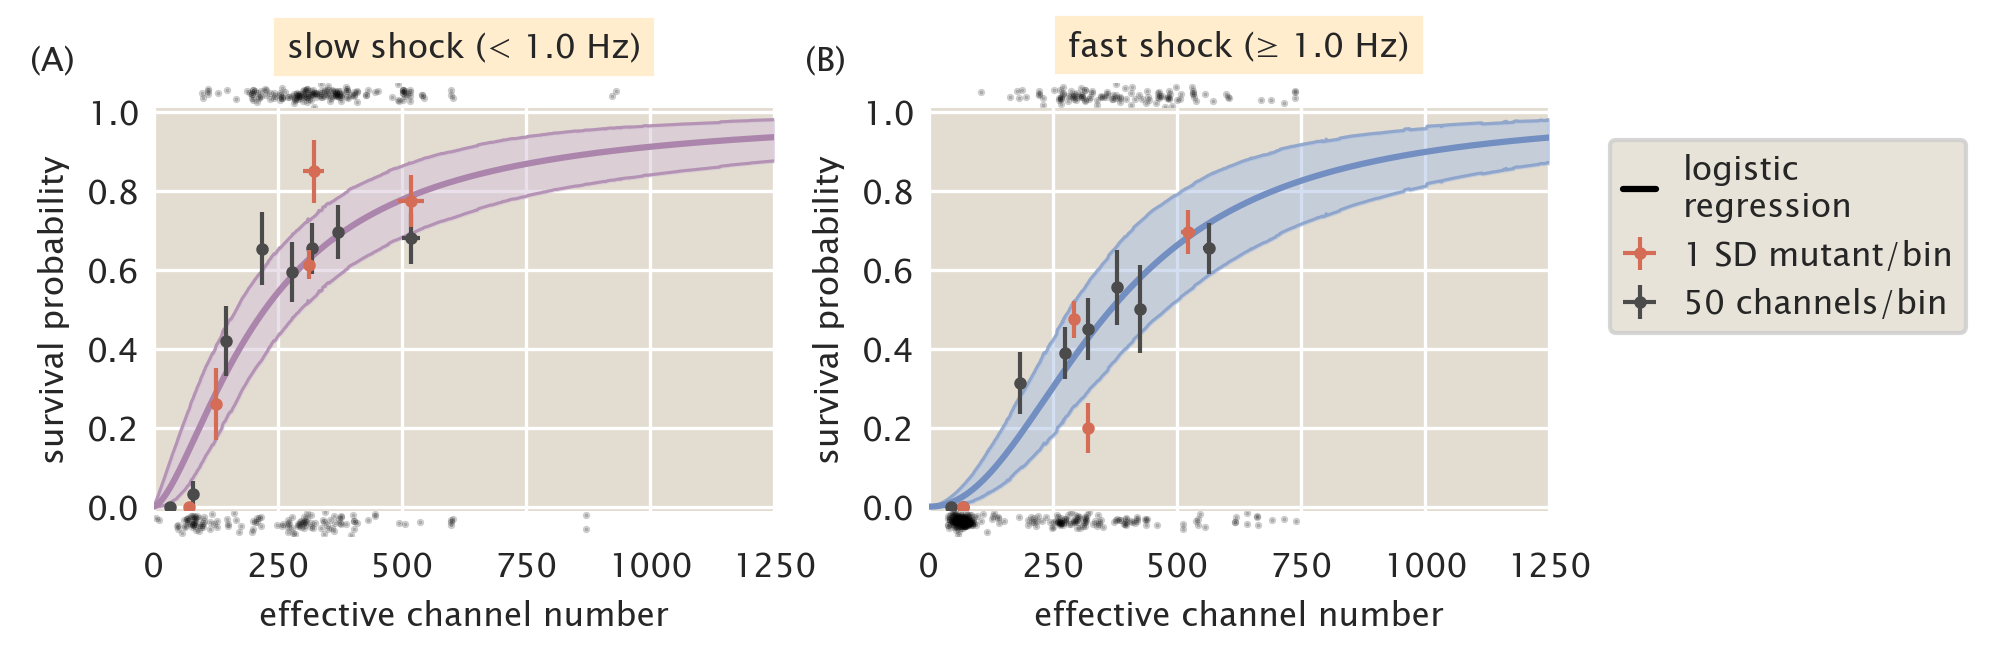
\includegraphics{../figs/fig5.pdf}
\caption{\textbf{Probability
of
survival
as a
function
of
MscL
copy
number.}
(A)
Estimated
survival
probability
for
survival
under
slow
shock
as a
function
of
channel
copy
number.
(B)
The
estimated
survival
probability
of
survival
under
a fast
shock
as a
function
of
channel
copy
number.
Solid
curves
correspond
to the
most
probable
survival
probability
from a
one-dimensional
logistic
regression.
Shaded
regions
represent
the
95\%
credible
regions.
Points
at the
top
and
bottom
of
plots
represent
individual
cell
measurements
which
survived
and
perished,
respectively.
The
red
and
black
points
correspond
to the
survival
probability
estimated
via
binning
by
Shine-Dalgarno
sequence
and
binning
by
groups
of 50
channels
per
cell,
respectively.
Horizontal
error
bars
represent
the
standard
error
of the
mean
from
at
least
25
measurements.
Vertical
error
bars
represent
the
certainty
of the
probability
estimate
given
\(n\)
survival
events
from
\(N\)
total
observations.}\label{fig:survival}
\end{figure}

\subsection{Discussion}\label{discussion}

~~~~One
of the
most
challenging
endeavors
in the
biological
sciences
is
linking
the
microscopic
details
of
cellular
components
to the
macro-scale
physiology
of the
organism.
This
formidable
task
has
been
met
repeatedly
in the
recent
history
of
biology,
especially
in the
era of
DNA
sequencing
and
single
molecule
biochemistry.
For
example,
the
scientific
community
has
been
able
to
connect
sickle-cell
anemia
to a
single
amino
acid
substitution
in
Hemoglobin
which
promotes
precipitation
under
a
change
in
O\(_2\)
partial
pressure
(\protect\hyperlink{ref-feeling-taylor2004}{23}--\protect\hyperlink{ref-perutz1950}{25}).
Others
have
assembled
a
physical
model
that
quantitatively
describes
chemosensation
in
bacteria
(\protect\hyperlink{ref-berg1977}{26})
in
which
the
arbiter
of
sensory
adaptation
is the
repeated
methylation
of
chemoreceptors
(\protect\hyperlink{ref-colin2017}{27}--\protect\hyperlink{ref-sourjik2002}{30}).
In the
past
\textasciitilde{}50
years
alone,
numerous
biological
and
physical
models
of the
many
facets
of the
central
dogma
have
been
assembled
that
give
us a
sense
of the
interplay
between
the
genome
and
physiology.
For
example,
the
combination
of
biochemical
experimentation
and
biophysical
models
have
given
us a
picture
of how
gene
dosage
affects
furrow
positioning
in
\emph{Drosophila}
(\protect\hyperlink{ref-liu2013}{31}),
how
recombination
of
V(D)J
gene
segments
generates
an
extraordinarily
diverse
antibody
repertoire
(\protect\hyperlink{ref-lovely2015}{32}--\protect\hyperlink{ref-schatz2011}{34}),
and
how
telomere
shortening
through
DNA
replication
is
intrinsically
tied
to
cell
senescence
(\protect\hyperlink{ref-herbig2004}{35},
\protect\hyperlink{ref-victorelli2017}{36}),
to
name
just a
few of
many
such
examples.

~~~~
By no
means
are we
``finished''
with
any of
these
topics.
Rather,
it's
quite
the
opposite
in the
sense
that
having
a
handle
on the
biophysical
knobs
that
tune
the
behavior
opens
the
door
to a
litany
of new
scientific
questions.
In the
case
of
mechanosenstaion
and
osmoregulation,
we
have
only
recently
been
able
to
determine
some
of the
basic
facts
that
allow
us to
approach
this
fascinating
biological
phenomenon
biophysically.
The
dependence
of
survival
on
mechanosensitive
channel
abundance
is a
key
quantity
that
is
missing
from
our
collection
of
critical
facts.
To our
knowledge,
this
work
represents
the
first
attempt
to
quantitatively
control
the
abundance
of a
single
species
of
mechanosensitive
channel
and
examine
the
physiological
consequences
in
terms
of
survival
probability
at
single-cell
resolution.
Our
results
reveal
two
notable
quantities.
First,
out of
the
several
hundred
single-cell
measurements,
we
never
observed
a cell
which
had
less
than
approximately
100
channels
per
cell
and
survived
an
osmotic
shock,
irrespective
of the
shock
rate.
The
second
is
that
between
500
and
700
channels
per
cell
are
needed
to
provide
\(\geq 80\%\)
survival,
depending
on the
shock
rate.

~~~~Only
recently
has
the
relationship
between
the
MscL
copy
number
and
the
probability
of
survival
been
approached
experimentally.
In van
den
Berg
et al.
(2016),
the
authors
examined
the
contribution
of
MscL
to
survival
in a
genetic
background
where
all
other
known
mechanosensitive
channels
had
been
deleted
from
the
chromosome
and
plasmid-borne
expression
of an
MscL-mEos3.2
fusion
was
tuned
through
an
IPTG
inducible
promoter
(\protect\hyperlink{ref-vandenberg2016}{8}).
In
this
work,
they
measured
the
single-cell
channel
abundance
through
super-resolution
microscopy
and
queried
survival
through
bulk
assays.
They
report
a
nearly
linear
relationship
between
survival
and
copy
number,
with
approximately
100
channels
per
cell
conveying
100\%
survival.
This
number
is
significantly
smaller
than
our
observation
of
approximately
100
channels
as the
\emph{minimum}
number
needed
to
convey
an y
observable
degree
of
survival.

~~~~
The
disagreement
between
the
numbers
reported
in
this
work
and in
van
den
Berg
et al.
may
partially
arise
from
subtle
differences
in the
experimental
approach.
The
primary
practical
difference
is the
magnitude
of the
osmotic
shock.
van
den
Berg
et al.
applied
an
approximately
600
mOsm
downshock
in
bulk
whereas
we
applied
a 1
Osm
downshock,
which
would
lead
to
lower
survival
(\protect\hyperlink{ref-levina1999}{37}).
In
their
work,
the
uncertainty
in
both
the
MscL
channel
count
and
survival
probability
is
roughly
30\%
(Fig.
S14).
Given
this
uncertainty,
it is
reasonable
to
interpret
that
the
number
of
channels
needed
for
complete
protection
from
osmotic
downshock
is
between
100
and
250
per
cell.
The
uncertainty
in
determining
the
number
of
channels
per
cell
is
consistent
with
the
observed
width
of the
channel
number
distribution
of the
Shine-Dalgarno
sequence
mutants
used
in
this
work
(Fig.~\ref{fig:boxplot}B).
A
unique
property
of the
single-cell
measurements
performed
in
this
work
allow
is the
direct
observation
of
survival
or
death
of
individual
cells.
We
find
that
morphological
classification
and
classification
through
a
propidium
iodide
staining
agree
within
1\%
(Supplement
C).
The
bulk
plating
assays,
as are
used
in van
den
Berg
et
al.,
rely
on
colony
formation
and
outgrowth
to
determine
survival
probability.
As is
reported
in
their
supplemental
information,
the
precision
in
this
measurement
is
around
30\%
(Fig.
S14).
Accounting
for
this
uncertainty
brings
both
measurements
within
a few
fold
where
we
still
consistently
observe
lower
survival
for a
given
channel
number.
This
remaining
disagreement
may be
accounted
for by
systematic
uncertainty
in
both
experimental
methods.

~~~~For
example,
variation
in the
length
of
outgrowth,
variable
shock
rate,
and
counting
statistics
could
bias
towards
higher
observed
survival
rates
in
ensemble
plating
assays.
During
the
outgrowth
phase,
the
control
sample
not
exposed
to an
osmotic
shock
is
allowed
to
grow
for
approximately
30
minutes
in a
high-salt
medium
before
plating.
The
shocked
cells,
however,
are
allowed
to
grow
in a
low-salt
medium.
We
have
found
that
the
difference
between
the
growth
rates
in
these
two
conditions
can be
appreciable
(approximately
35
minutes
versus
20
minutes,
respectively)
as can
be
seen
in Fig
S2.
Cells
that
survived
an
osmotic
shock
may
have a
growth
advantage
relative
to the
control
sample
if the
shock-induced
lag
phase
is
less
than
the
outgrowth,
leading
to
higher
observed
survival
rates
(\protect\hyperlink{ref-levina1999}{37}).
This
is one
possible
explanation
for
the
survival
rates
which
are
reported
in
excess
of
100\%.
Cells
that
survived
an
osmotic
shock
may
have a
growth
advantage
relative
to the
normalization
sample
if the
shock-induced
lag
phase
is
less
than
the
outgrowth,
leading
to
higher
observed
survival
rates,
even
surpassing
100\%.
We
have
performed
these
assays
ourselves
and
have
observed
survival
rates
above
of
100\%
(ranging
from
110\%
to
125\%)
with
an
approximate
30\%
error
(see
Fig.
S3 in
Bialecka-Fornal
et al.
2012
(\protect\hyperlink{ref-bialecka-fornal2012}{3}))
which
we
concluded
to
arise
from
differences
in
growth
rate.
We
also
note
that
survival
rates
greater
than
100\%
are
observed
in van
den
Berg
et al.
(Fig.
S14).
For
strains
that
have
survival
rates
between
80\%
and
100\%
the
uncertainty
is
typically
large,
making
it
difficult
to
make
precise
statements
regarding
when
full
survival
is
achieved.

~~~~It
has
been
shown
that
there
is a
strong
inverse
relationship
between
the
rate
of
osmotic
shock
and
survival
probability
(\protect\hyperlink{ref-bialecka-fornal2015}{4}).
Any
experiment
in
which
the
shock
was
applied
more
slowly
or
quickly
than
another
would
bias
toward
higher
or
lower
survivability,
respectively.
The
shocks
applied
in
bulk
assays
are
often
performed
manually
which
can be
highly
variable.
We
note
that
in our
experiments,
we
frequently
observe
cells
which
do not
separate
and
form
chains
of two
or
more
cells
(Fig.
S9 and
S10).
In
plating
assays,
it is
assumed
that
colonies
arise
from a
single
founding
cell
however
a
colony
formed
by a
cluster
of
living
and
dead
cells
would
be
interpreted
as a
single
surviving
cell,
effectively
masking
the
death
of the
others
in the
colony
forming
unit.
This
too
could
bias
the
measurement
toward
higher
survival
rates.
Single-cell
shock
experiments
can
also
have
systematic
errors
which
can
bias
the
results
towards
lower
survival
rates.
Such
errors
are
associated
with
handling
of the
cells
such
as
shear
damage
from
loading
into
the
flow
cell,
adhering
the
cells
to the
coverslip,
and
any
chemical
perturbations
introduced
by the
dye
used
to
measure
the
shock
rate.

~~~~Despite
these
experimental
differences,
the
results
of
this
work
and
van
den
Berg
et
al.,
are in
agreement
that
MscL
must
be
present
at the
level
of 100
or
more
channels
per
cell
in
wild-type
cells
to
convey
appreciable
survival.
As
both
of
these
works
were
performed
in a
strain
in
which
the
only
mechanosensitive
channel
was
MscL,
it
remains
unknown
how
the
presence
of the
other
channel
species
would
alter
the
number
of
MscL
needed
for
complete
survival.
In our
experiments,
we
observed
a
maximum
survival
probability
of
approximately
80\%
even
with
close
to
1000
MscL
channels
per
cell.
It is
possible
that
the
combined
effort
of the
six
other
mechanosensitive
channels
would
make
up for
some
if not
all of
the
remaining
20\%.
To
explore
the
contribution
of
another
channel
to
survival,
van
den
Berg
et al.
also
queried
the
contribution
of
MscS,
another
mechanosensitive
channel,
to
survival
in the
absence
of any
other
species
of
mechansensitive
channel.
It was
found
that
over
the
explored
range
of
MscS
channel
copy
numbers,
the
maximum
survival
rate
was
approximately
50\%,
suggesting
that
different
mechanosensitive
channels
have
an
upper
limit
to how
much
protection
they
can
confer.
Both
van
den
Berg
et al.
and
our
work
show
that
there
is
still
much
to be
learned
with
respect
to the
interplay
between
the
various
species
of
mechanosensitive
channel
as
well
as
their
regulation.

~~~~
Recent
work
has
shown
that
both
magnitude
and
the
rate
of
osmotic
down
shock
are
important
factors
in
determining
cell
survival
(\protect\hyperlink{ref-bialecka-fornal2015}{4}).
In
this
work,
we
show
that
this
finding
holds
true
for a
single
species
of
mechanosensitive
channel,
even
at
high
levels
of
expression.
One
might
naïvely
expect
that
this
rate-dependent
effect
would
disappear
once a
certain
threshold
of
channels
had
been
met.
Our
experiments,
however,
show
that
even
at
nearly
1000
channels
per
cell
the
predicted
survival
curves
for a
slow
(\(< 1.0\)
Hz)
and
fast
(\(\geq 1.0\)
Hz)
are
shifted
relative
to
each
other
with
the
fast
shock
predicting
lower
rates
of
survival.
This
suggests
either
we
have
not
reached
this
threshold
in our
experiments
or
there
is
more
to
understand
about
the
relationship
between
abundance,
channel
species,
and
the
shock
rate.

~~~~
Some
experimental
and
theoretical
treatments
suggest
that
only a
few
copies
of
MscL
or
MscS
should
be
necessary
for
100\%
protection
given
our
knowledge
of the
conductance
and
the
maximal
water
flux
through
the
channel
in its
open
state
(\protect\hyperlink{ref-louhivuori2010}{11},
\protect\hyperlink{ref-booth2014}{38}).
However,
recent
proteomic
studies
have
revealed
average
MscL
copy
numbers
to be
in the
range
of
several
hundred
per
cell,
depending
on the
condition,
as can
be
seen
in
Table
1
(\protect\hyperlink{ref-schmidt2016}{15},
\protect\hyperlink{ref-soufi2015}{16},
\protect\hyperlink{ref-li2014}{39}).
Studies
focusing
solely
on
MscL
have
shown
similar
counts
through
quantitative
Western
blotting
and
fluorescence
microscopy
(\protect\hyperlink{ref-bialecka-fornal2012}{3}).
Electrophysiology
studies
have
told
another
story
with
copy
number
estimates
ranging
between
4 and
100
channels
per
cell
(\protect\hyperlink{ref-stokes2003a}{17},
\protect\hyperlink{ref-blount1999}{40}).
These
measurements,
however,
measure
the
active
number
of
channels.
The
factors
regulating
channel
activity
in
these
experiments
could
be due
to
perturbations
during
the
sample
preparation
or
reflect
some
unknown
mechanism
of
regulation,
such
as the
presence
or
absence
of
interacting
cofactors
(\protect\hyperlink{ref-schumann2010}{41}).
The
work
described
here,
on the
other
hand,
measures
the
\emph{maximum}
number
of
channels
that
could
be
active
and
may be
able
to
explain
why
the
channel
abundance
is
higher
than
estimated
by
theoretical
means.
There
remains
much
more
to be
learned
about
the
regulation
of
activity
in
these
systems.
As the
\emph{in
vivo}
measurement
of
protein
copy
number
becomes
accessible
through
novel
single-cell
and
single-molecule
methods,
we
will
continue
to
collect
more
facts
about
this
fascinating
system
and
hopefully
connect
the
molecular
details
of
mechanosensation
with
perhaps
the
most
important
physiological
response
--
life
or
death.

\begin{longtable}[]{@{}llc@{}}
\caption{Measured
cellular
copy
numbers
of
MscL.
Asterisk
(*)
Indicates
inferred
MscL
channel
copy
number
from
the
total
number
of
detected
MscL
peptides.}\tabularnewline
\toprule
\begin{minipage}[b]{0.29\columnwidth}\raggedright\strut
Reported
channels
per
cell\strut
\end{minipage}
&
\begin{minipage}[b]{0.29\columnwidth}\raggedright\strut
Method\strut
\end{minipage}
&
\begin{minipage}[b]{0.34\columnwidth}\centering\strut
Reference\strut
\end{minipage}\tabularnewline
\midrule
\endfirsthead
\toprule
\begin{minipage}[b]{0.29\columnwidth}\raggedright\strut
Reported
channels
per
cell\strut
\end{minipage}
&
\begin{minipage}[b]{0.29\columnwidth}\raggedright\strut
Method\strut
\end{minipage}
&
\begin{minipage}[b]{0.34\columnwidth}\centering\strut
Reference\strut
\end{minipage}\tabularnewline
\midrule
\endhead
\begin{minipage}[t]{0.29\columnwidth}\raggedright\strut
480 ±
103\strut
\end{minipage}
&
\begin{minipage}[t]{0.29\columnwidth}\raggedright\strut
Western
blotting\strut
\end{minipage}
&
\begin{minipage}[t]{0.34\columnwidth}\centering\strut
(\protect\hyperlink{ref-bialecka-fornal2012}{3})\strut
\end{minipage}\tabularnewline
\begin{minipage}[t]{0.29\columnwidth}\raggedright\strut
560*\strut
\end{minipage}
&
\begin{minipage}[t]{0.29\columnwidth}\raggedright\strut
Ribosomal
profiling\strut
\end{minipage}
&
\begin{minipage}[t]{0.34\columnwidth}\centering\strut
(\protect\hyperlink{ref-li2014}{39})\strut
\end{minipage}\tabularnewline
\begin{minipage}[t]{0.29\columnwidth}\raggedright\strut
331*\strut
\end{minipage}
&
\begin{minipage}[t]{0.29\columnwidth}\raggedright\strut
Mass
spectrometry\strut
\end{minipage}
&
\begin{minipage}[t]{0.34\columnwidth}\centering\strut
(\protect\hyperlink{ref-schmidt2016}{15})\strut
\end{minipage}\tabularnewline
\begin{minipage}[t]{0.29\columnwidth}\raggedright\strut
583*\strut
\end{minipage}
&
\begin{minipage}[t]{0.29\columnwidth}\raggedright\strut
Mass
spectrometry\strut
\end{minipage}
&
\begin{minipage}[t]{0.34\columnwidth}\centering\strut
(\protect\hyperlink{ref-soufi2015}{16})\strut
\end{minipage}\tabularnewline
\begin{minipage}[t]{0.29\columnwidth}\raggedright\strut
4 -
5\strut
\end{minipage}
&
\begin{minipage}[t]{0.29\columnwidth}\raggedright\strut
Electrophysiology\strut
\end{minipage}
&
\begin{minipage}[t]{0.34\columnwidth}\centering\strut
(\protect\hyperlink{ref-stokes2003a}{17})\strut
\end{minipage}\tabularnewline
\begin{minipage}[t]{0.29\columnwidth}\raggedright\strut
10 -
100\strut
\end{minipage}
&
\begin{minipage}[t]{0.29\columnwidth}\raggedright\strut
Electrophysiology\strut
\end{minipage}
&
\begin{minipage}[t]{0.34\columnwidth}\centering\strut
(\protect\hyperlink{ref-booth2005}{13})\strut
\end{minipage}\tabularnewline
\begin{minipage}[t]{0.29\columnwidth}\raggedright\strut
10 -
15\strut
\end{minipage}
&
\begin{minipage}[t]{0.29\columnwidth}\raggedright\strut
Electrophysiology\strut
\end{minipage}
&
\begin{minipage}[t]{0.34\columnwidth}\centering\strut
(\protect\hyperlink{ref-blount1999}{40})\strut
\end{minipage}\tabularnewline
\bottomrule
\end{longtable}

\subsection{Materials
\&
Methods}\label{materials-methods}

\subsubsection{Bacterial
strains
and
growth
conditions}\label{bacterial-strains-and-growth-conditions}

The
bacterial
strains
are
described
in
Table
S3.
The
parent
strain
for
the
mutants
used
in
this
study
was
MJF641
(\protect\hyperlink{ref-edwards2012}{5})
(generously
provided
by
Drs.
Samantha
Miller
and
Ian
Booth),
a
strain
which
had
all
seven
mechanosensitive
channels
deleted.
The
MscL-sfGFP
coding
region
from
MLG910
(\protect\hyperlink{ref-bialecka-fornal2012}{3})
was
integrated
into
MJF641
by P1
transduction,
creating
the
strain
D6LG-Tn10.
Selection
pressure
for
MscL
integration
was
created
by
incorporating
an
osmotic
shock
into
the
transduction
protocol,
which
favored
the
survival
of
MscL-expressing
stains
relative
to
MJF641
by
\textasciitilde{}100-fold.
Screening
for
integration
candidates
was
based
on
fluorescence
expression
of
plated
colonies.
Successful
integration
was
verified
by
sequencing.
Attempts
to
transduce
RBS-modified
MscL-sfGFP
coding
regions
became
increasingly
inefficient
as the
targeted
expression
level
of
MscL
was
reduced.
This
was
due to
the
decreasing
fluorescence
levels
and
survival
rates
of the
integration
candidates.
Consequently,
Shine-Dalgarno
sequence
modifications
were
made
by
inserting
DNA
oligos
with
lambda
red-mediated
homologous
recombination,
i.e.,
recombineering
(\protect\hyperlink{ref-sharan2009}{42}).
The
oligos
had a
designed
mutation
(Fig.~\ref{fig:boxplot})
flanked
by
\textasciitilde{}25
base
pairs
that
matched
the
targeted
MscL
region
(Table
S4). A
two-step
recombineering
process
of
selection
followed
by
counter
selection
using
a
\emph{tetA-sacB}
gene
fusion
cassette
(\protect\hyperlink{ref-li2013}{43})
was
chosen
because
of its
capabilities
to
integrate
with
efficiencies
comparable
to P1
transduction
and
not
leave
antibiotic
resistance
markers
or
scar
sequences
in the
final
strain.
To
prepare
the
strain
D6LG-Tn10
for
this
scheme,
the
Tn10
transposon
containing
the
\emph{tetA}
gene
needed
to be
removed
to
avoid
interference
with
the
\emph{tetA-sacB}
cassette.
Tn10
was
removed
from
the
middle
of the
\emph{ycjM}
gene
with
the
primer
Tn10delR
(Table
S2) by
recombineering,
creating
the
strain
D6LG
(SD0).
Counter
selection
against
the
\emph{tetA}
gene
was
promoted
by
using
agar
media
with
fusaric
acid
(\protect\hyperlink{ref-li2013}{43},
\protect\hyperlink{ref-bochner1980}{44}).
The
\emph{tetA-sacB}
cassette
was
PCR
amplified
out of
the
strain
XTL298
using
primers
MscLSPSac
and
MscLSPSacR
(Table
S2).
The
cassette
was
integrated
in
place
of the
spacer
region
in
front
of the
MscL
start
codon
of
D6LG
(SD0)
by
recombineering,
creating
the
intermediate
strain
D6LTetSac.
Positive
selection
for
cassette
integration
was
provided
by
agar
media
with
tetracycline.
Finally,
the
RBS
modifying
oligos
were
integrated
into
place
by
replacing
the
\emph{tetA-sacB}
cassette
by
recombineering.
Counter
selection
against
both
\emph{tetA}
and
\emph{sacB}
was
ensured
by
using
agar
media
with
fusaric
acid
and
sucrose
(\protect\hyperlink{ref-li2013}{43}),
creating
the
Shine-Dalgarno
mutant
strains
used
in
this
work.

Strain
cultures
were
grown
in 5
mL of
LB-Lennox
media
with
antibiotic
(apramycin)
overnight
at
37°C.
The
next
day,
50 µL
of
overnight
culture
was
inoculated
into 5
mL of
LB-Lenox
with
antibiotic
and
the
culture
was
grown
to
OD600nm
\textasciitilde{}0.25.
Subsequently,
500 µL
of
that
culture
was
inoculated
into 5
mL of
LB-Lennox
supplemented
with
500mM
of
NaCl
and
the
culture
was
regrown
to
OD600nm
\textasciitilde{}0.25.
A 1 mL
aliquot
was
taken
and
used
to
load
the
flow
cell.

\subsubsection{Flow
cell}\label{flow-cell}

~ ~ ~
~ All
experiments
were
conducted
in a
home-made
flow
cell
as is
shown
in
Fig.~\ref{fig:flow_cell}A.
This
flow
cell
has
two
inlets
which
allow
media
of
different
osmolarity
to be
exchanged
over
the
course
of the
experiment.
The
imaging
region
is
approximately
10 mm
wide
and
100
\(\mu\)m
in
depth.
All
imaging
took
place
within
1 -- 2
cm of
the
outlet
to
avoid
imaging
cells
within
a
non-uniform
gradient
of
osmolarity.
The
interior
of the
flow
cell
was
functionalized
with a
1:400
dilution
of
polyethylenimine
prior
to
addition
of
cells
with
the
excess
washed
away
with
water.
A
dilute
cell
suspension
in LB
Lennox
with
500 mM
NaCl
was
loaded
into
one
inlet
while
the
other
was
connected
to a
vial
of LB
medium
with
no
NaCl.
This
hypotonic
medium
was
clamped
during
the
loading
of the
cells.

~ ~ ~
~Once
the
cells
had
adhered
to the
polyethylenimine
coated
surface,
the
excess
cells
were
washed
away
with
the
500 mM
NaCl
growth
medium
followed
by a
small
(\textasciitilde{}20
\(\mu\)L)
air
bubble.
This
air
bubble
forced
the
cells
to lay
flat
against
the
imaging
surface,
improving
the
time-lapse
imaging.
Over
the
observation
period,
cells
not
exposed
to an
osmotic
shock
were
able
to
grow
for 4
-- 6
divisions,
showing
that
the
flow
cell
does
not
directly
impede
cell
growth.

\subsubsection{Imaging
conditions}\label{imaging-conditions}

~ ~ ~
~All
imaging
was
performed
in a
flow
cell
held
at
30°C
on a
Nikon
Ti-Eclipse
microscope
outfitted
with a
Perfect
Focus
system
enclosed
in a
Haison
environmental
chamber
(approximately
1°C
regulation
efficiency).
The
microscope
was
equipped
with a
488 nm
laser
excitation
source
(CrystaLaser)
and a
520/35
laser
optimized
filter
set
(Semrock).
The
images
were
collected
on an
Andor
iXon
EM+
897
EMCCD
camera
and
all
microscope
and
acquisition
operations
were
controlled
via
the
open
source
\(\mu\)Manager
microscope
control
software
(\protect\hyperlink{ref-edelstein2014}{45}).
Once
cells
were
securely
mounted
onto
the
surface
of the
glass
coverslip,
between
15 and
20
positions
containing
5 to
10
cells
were
marked
and
the
coordinates
recorded.
At
each
position,
a
phase
contrast
and
GFP
fluorescence
image
was
acquired
for
segmentation
and
subsequent
measurement
of
channel
copy
number.
To
perform
the
osmotic
shock,
LB
media
containing
no
NaCl
was
pulled
into
the
flow
cell
through
a
syringe
pump.
To
monitor
the
media
exchange,
both
the
high
salt
and no
salt
LB
media
were
supplemented
with a
low-affinity
version
of the
calcium-sensitive
dye
Rhod-2
(250
nM;
TEF
Labs)
which
fluoresces
when
bound
to
Ca\textsuperscript{2+}.
The no
salt
medium
was
also
supplemented
with
1\(\mu\)M
CaCl\(_2\)
to
make
the
media
mildly
fluorescent
and
the
exchange
rate
was
calculated
by
measuring
the
fluorescence
increase
across
an
illuminated
section
of one
of the
positions.
These
images
were
collected
in
real
time
for
the
duration
of the
shock.
The
difference
in
measured
fluorescence
between
the
pre-shock
images
and
those
at the
end of
the
shock
set
the
scale
of a
500 mM
NaCl
down
shock.
The
rate
was
calculated
by
fitting
a line
to the
middle
region
of
this
trace.
Further
details
regarding
this
procedure
can be
found
in
Bialecka-Fornal
et al.
2015
(\protect\hyperlink{ref-bialecka-fornal2015}{4}).

\subsubsection{Image
Processing}\label{image-processing}

~ ~ ~
~Images
were
processed
using
a
combination
of
automated
and
manual
methods.
First,
expression
of
MscL
was
measured
via
segmenting
individual
cells
or
small
clusters
of
cells
in
phase
contrast
and
computing
the
mean
pixel
value
of the
fluorescence
image
for
each
segmented
object.
The
fluorescence
images
were
passed
through
several
filtering
operations
which
reduced
high-frequency
noise
as
well
as
corrected
for
uneven
illumination
of the
excitation
wavelength.

~ ~ ~
~Survival
or
death
classification
was
performed
manually
using
the
CellProfiler
plugin
for
ImageJ
software
(NIH).
A
survivor
was
defined
as a
cell
which
was
able
to
undergo
at
least
two
division
events
after
the
osmotic
down
shock.
Cell
death
was
recognized
by
stark
changes
in
cell
morphology
including
loss
of
phase
contrast
through
ejection
of
cytoplasmic
material,
structural
decomposition
of the
cell
wall
and
membrane,
and
the
inability
to
divide.
To
confirm
that
these
morphological
cues
corresponded
with
cell
death,
we
probed
cell
viability
on a
subset
of our
strains
after
osmotic
shock
through
staining
with
propidium
iodide,
a DNA
intercalating
dye
commonly
used
to
identifying
dead
cells
(LIVE/DEAD
BacLight
Bacterial
Cell
Viability
Assay,
Thermo
Fisher).
We
found
that
our
classification
based
on
morphology
agreed
with
that
based
off of
staining
within
1\%.
More
information
regarding
these
experiments
can be
found
in the
Supplement
C.
Cells
which
detached
from
the
surface
during
the
post-shock
growth
phase
or
those
which
became
indistinguishable
from
other
cells
due to
clustering
were
not
counted
as
survival
or
death
and
were
removed
from
the
dataset
completely.
A
region
of the
cell
was
manually
marked
with
1.0
(survival)
or 0.0
(death)
by
clicking
on the
image.
The
\texttt{xy}
coordinates
of the
click
as
well
as the
assigned
value
were
saved
as an
\texttt{.xml}
file
for
that
position.

~ ~ ~
~The
connection
between
the
segmented
cells
and
their
corresponding
manual
markers
was
automated.
As the
manual
markings
were
made
on the
first
phase
contrast
image
after
the
osmotic
shock,
small
shifts
in the
positions
of the
cell
made
one-to-one
mapping
with
the
segmentation
mask
non-trivial.
The
linkages
between
segmented
cell
and
manual
marker
were
made
by
computing
all
pairwise
distances
between
the
manual
marker
and
the
segmented
cell
centroid,
taking
the
shortest
distance
as the
true
pairing.
The
linkages
were
then
inspected
manually
and
incorrect
mappings
were
corrected
as
necessary.

~ ~ ~
~All
relevant
statistics
about
the
segmented
objects
as
well
as the
sample
identity,
date
of
acquisition,
osmotic
shock
rate,
and
camera
exposure
time
were
saved
as
\texttt{.csv}
files
for
each
individual
experiment.
A more
in-depth
description
of the
segmentation
procedure
as
well
as the
relevant
code
can be
accessed
as a
Jupyter
Notebook
at
(\texttt{http://rpgroup.caltech.edu/mscl\_survival}).

\subsubsection{Calculation
of
effective
channel
copy
number}\label{calculation-of-effective-channel-copy-number}

~ ~ ~
~To
compute
the
MscL
channel
copy
number,
we
relied
on
measuring
the
fluorescence
level
of a
bacterial
strain
in
which
the
mean
MscL
channel
copy
number
was
known
via
fluorescence
microscopy
(\protect\hyperlink{ref-bialecka-fornal2012}{3}).
\emph{E.
coli}
strain
MLG910,
which
expresses
the
MscL-sfGFP
fusion
protein
from
the
wild-type
SD
sequence,
was
grown
under
identical
conditions
to
those
described
in
Bialecka-Fornal
et al.
2015
in LB
Miller
medium
(BD
Medical
Sciences)
to an
OD\textsubscript{600nm}
of
\textasciitilde{}0.3.
The
cells
were
then
diluted
ten
fold
and
immobilized
on a
rigid
2\%
agarose
substrate
and
placed
onto a
glass
bottom
petri
dish
and
imaged
in the
same
conditions
as
described
previously.

~ ~
~Images
were
taken
of six
biological
replicates
of
MLG910
and
were
processed
identically
to
those
in the
osmotic
shock
experiments.
A
calibration
factor
between
the
average
cell
fluorescence
level
and
mean
MscL
copy
number
was
then
computed.
We
assumed
that
all
measured
fluorescence
(after
filtering
and
background
subtraction)
was
derived
from
the
MscL-sfGFP
fusion,
\begin{equation}
\langle I_\text{tot}\rangle = \alpha \langle N \rangle,
\label{eq:ian}\end{equation}
in
which
\(\alpha\)
is the
calibration
factor
and
\(\langle N \rangle\)
is the
mean
cellular
MscL-sfGFP
copy
number
as
reported
in
Bialecka-Fornal
et al.
2012
(\protect\hyperlink{ref-bialecka-fornal2012}{3}).
To
correct
for
errors
in
segmentation,
the
intensity
was
computed
as an
areal
density
\(\langle I_A \rangle\)
and
was
multiplied
by the
average
cell
area
\(\langle A \rangle\)
of the
population.
The
calibration
factor
was
therefore
computed
as
\begin{equation}
\alpha = {\langle I_A \rangle \langle A \rangle \over \langle N \rangle}.
\label{eq:calibration_factor}\end{equation}

~~~We
used
Bayesian
inferential
methods
to
compute
this
calibration
factor
taking
measurement
error
and
replicate-to-replicate
variation
into
account.
The
resulting
average
cell
area
and
calibration
factor
was
used
to
convert
the
measured
cell
intensities
from
the
osmotic
shock
experiments
to
cell
copy
number.
The
details
of
this
inference
are
described
in
depth
in the
supplemental
information
(\emph{Standard
Candle
Calibration}).

\subsubsection{Logistic
regression}\label{logistic-regression}

~ ~ ~
~We
used
Bayesian
inferential
methods
to
find
the
most
probable
values
of the
coefficients
\(\beta_0\)
and
\(\beta_1\)
and
the
appropriate
credible
regions
and is
described
in
detail
in the
supplemental
information
(\emph{Logistic
Regression}).
Briefly,
we
used
Markov
chain
Monte
Carlo
(MCMC)
to
sample
from
the
log
posterior
distribution
and
took
the
most
probable
value
as the
mean
of the
samples
for
each
parameter.
The
MCMC
was
performed
using
the
Stan
probabilistic
programming
language
(\protect\hyperlink{ref-carpenter2017}{46})
and
all
models
can be
found
on the
GitHub
repository
(\texttt{http://github.com/rpgroup-pboc/mscl\_survival}).

\subsubsection{Calculation
of
survival
probability
error}\label{calculation-of-survival-probability-error}

~~~~The
vertical
error
bars
for
the
points
shown
in
Fig.~\ref{fig:survival}
represent
our
uncertainty
in the
survival
probability
given
our
measurement
of
\(n\)
survivors
out of
a
total
\(N\)
single-cell
measurements.
The
probability
distribution
of the
survival
probability
\(p_s\)
given
these
measurements
can be
written
using
Bayes'
theorem
as
\begin{equation}
g(p_s\,\vert\, n, N) = {f(n\,\vert\,p_s, N)g(p_s) \over f(n\,\vert\, N)},
\label{eq:probability_bayes}\end{equation}
where
\(g\)
and
\(f\)
represent
probability
density
functions
over
parameters
and
data,
respectively.
The
likelihood
\(f(n\,\vert p_s, N)\)
represents
the
probability
of
measuring
\(n\)
survival
events,
given
a
total
of
\(N\)
measurements
each
with a
probability
of
survival
\(p_s\).
This
matches
the
story
for
the
Binomial
distribution
and
can be
written
as
\begin{equation}
f(n\,\vert\,p_s, N) = {N! \over n!(N - n)!}p_s^n(1 - p_s)^{N - n}.
\label{eq:binomial}\end{equation}
To
maintain
maximal
ignorance
we can
assume
that
any
value
for
\(p_s\)
is
valid,
such
that
is in
the
range
{[}0,
1{]}.
This
prior
knowledge,
represented
by
\(g(p_s)\),
can be
written
as
\begin{equation}
g(p_s) = \begin{cases}1 & 0\leq p_s\leq 1 \\
0 & \text{otherwise} \end{cases}.
\label{eq:uniform_prob}\end{equation}
We can
also
assume
maximal
ignorance
for
the
total
number
of
survival
events
we
could
measure
given
\(N\)
observations,
\(f(n\, \vert\, N)\).
Assuming
all
observations
are
equally
likely,
this
can be
written
as
\begin{equation}
f(n\,\vert\, N) = {1 \over N + 1}
\label{eq:evidence}\end{equation}
where
the
addition
of one
comes
from
the
possibility
of
observing
zero
survival
events.
Combining
Eqns.~\ref{eq:binomial}, \ref{eq:uniform_prob}, \ref{eq:evidence},
the
posterior
distribution
\(g(p_s\,\vert\, n, N)\)
is
\begin{equation}
g(p_s\,\vert\, n, N) = {(N+1)! \over n!(N - n)!}p_s^{n}(1 - p_s)^{N - n}.
\label{eq:probability_posterior}\end{equation}

~~~~
The
most
probable
value
of
\(p_s\),
where
the
posterior
probability
distribution
given
by
Eq.~\ref{eq:probability_posterior}
is
maximized,
can be
found
by
computing
the
point
at
which
derivative
of the
log
posterior
with
respect
to
\(p_s\)
goes
to
zero,
\begin{equation}
{d\log g(p_s\,\vert\,n, N) \over d p_s} = {n \over p_s} - {N - n  \over 1 - p_s} = 0.
\label{eq:deriv_ps}\end{equation}
Solving
Eq.~\ref{eq:deriv_ps}
for
\(p_s\)
gives
the
most
likely
value
for
the
probability,
\begin{equation}
p_s^* = {n \over N}.
\label{eq:most_prob_prob}\end{equation}
So
long
as
\(N >> np_s^*\),
Eq.~\ref{eq:probability_posterior}
can be
approximated
as a
Gaussian
distribution
with a
mean
\(p_s^*\)
and a
variance
\(\sigma_{p_s}^2\).
By
definition,
the
variance
of a
Gaussian
distribution
is
computed
as the
negative
reciprocal
of the
second
derivative
of the
log
posterior
evaluated
at
\(p_s = p_s^*\),
\begin{equation}
\sigma_{p_s}^2 = - \left({d^2 \log g(p_s\,\vert\, n, N) \over dp_s^2}\Bigg\vert_{p_s=p_s^*}\right)^{-1}.
\label{eq:variance_def}\end{equation}
Evaluating
Eq.~\ref{eq:variance_def}
yields
\begin{equation}
\sigma_{p_s}^2 = {n(N-n)\over N^3}.
\label{eq:prob_variance}\end{equation}
Given
Eq.~\ref{eq:most_prob_prob}
and
Eq.~\ref{eq:prob_variance},
the
most-likely
survival
probability
and
estimate
of the
uncertainty
can be
expressed
as
\begin{equation}
p_s = p_s^* \pm \sigma_{p_s}.
\end{equation}

\subsubsection{Data
and
software
availability}\label{data-and-software-availability}

~ ~ ~
~All
raw
image
data
is
freely
available
and is
stored
on the
CaltechDATA
Research
Data
Repository
(\protect\hyperlink{ref-chure2018a}{47}).
The
raw
Markov
chain
Monte
Carlo
samples
are
stored
as
\texttt{.csv}
files
on
CaltechDATA
(\protect\hyperlink{ref-chure2018}{48}).
All
processed
experimental
data,
Python,
and
Stan
code
used
in
this
work
are
freely
available
through
our
GitHub
repository
(\texttt{http://github.com/rpgroup-pboc/mscl\_survival})(\protect\hyperlink{ref-chure2018b}{49})
accessible
through
DOI:
10.5281/zenodo.1252524.
The
scientific
community
is
invited
to
fork
our
repository
and
open
constructive
issues.

\subsection{Acknowledgements}\label{acknowledgements}

~ ~ ~
~We
thank
Nathan
Belliveau,
Maja
Bialecka-Fornal,
Justin
Bois,
Soichi
Hirokawa,
Jaspar
Landman,
Manuel
Razo-Mejia,
Muir
Morrison,
and
Shyam
Saladi
for
useful
advice
and
discussion.
We
thank
Prof.~Don
Court
for
strain
XTL298
as
well
as
Dr.~Samantha
Miller
and
Prof.~Ian
Booth
at the
University
of
Aberdeen
for
strain
MJF641.
This
work
was
supported
by the
National
Institutes
of
Health
DP1
OD000217
(Director's
Pioneer
Award),
R01
GM085286,
GM084211-A1
,
GM118043-01,
and La
Fondation
Pierre
Gilles
de
Gennes.

\subsection*{References}\label{references}
\addcontentsline{toc}{subsection}{References}

\hypertarget{refs}{}
\hypertarget{ref-martinac1987}{}
1.
Martinac
B,
Buechner
M,
Delcour
AH,
Adler
J,
Kung
C.
1987.
Pressure-sensitive
ion
channel
in
\emph{Escherichia
coli}.
Proc
Natl
Acad
Sci U
S A
84:2297--301.

\hypertarget{ref-bavi2016}{}
2.
Bavi
N,
Cortes
DM,
Cox
CD,
Rohde
PR,
Liu W,
Deitmer
JW,
Bavi
O,
Strop
P,
Hill
AP,
Rees
D,
Corry
B,
Perozo
E,
Martinac
B.
2016.
The
role
of
MscL
amphipathic
N
terminus
indicates
a
blueprint
for
bilayer-mediated
gating
of
mechanosensitive
channels.
Nature
Communications
7:11984.

\hypertarget{ref-bialecka-fornal2012}{}
3.
Bialecka-Fornal
M, Lee
HJ,
DeBerg
HA,
Gandhi
CS,
Phillips
R.
2012.
Single-Cell
Census
of
Mechanosensitive
Channels
in
Living
Bacteria.
PLoS
ONE
7:e33077.

\hypertarget{ref-bialecka-fornal2015}{}
4.
Bialecka-Fornal
M, Lee
HJ,
Phillips
R.
2015.
The
Rate
of
Osmotic
Downshock
Determines
the
Survival
Probability
of
Bacterial
Mechanosensitive
Channel
Mutants.
Journal
of
Bacteriology
197:231--237.

\hypertarget{ref-edwards2012}{}
5.
Edwards
MD,
Black
S,
Rasmussen
T,
Rasmussen
A,
Stokes
NR,
Stephen
TL,
Miller
S,
Booth
IR.
Jul-Aug
20122012.
Characterization
of
three
novel
mechanosensitive
channel
activities
in
Escherichia
coli.
Channels
(Austin)
6:272--81.

\hypertarget{ref-naismith2012}{}
6.
Naismith
JH,
Booth
IR.
2012.
Bacterial
mechanosensitive
channels--MscS:
Evolution's
solution
to
creating
sensitivity
in
function.
Annu
Rev
Biophys
41:157--77.

\hypertarget{ref-ursell2008}{}
7.
Ursell
T,
Phillips
R,
Kondev
J,
Reeves
D,
Wiggins
PA.
2008.
The
role
of
lipid
bilayer
mechanics
in
mechanosensation,
pp.
37--70.
\emph{In}
Kamkin,
A,
Kiseleva,
I
(eds.),
Mechanosensitivity
in
cells
and
tissues
1:
Mechanosensitive
ion
channels.
Springer-Verlag.

\hypertarget{ref-vandenberg2016}{}
8. van
den
Berg
J,
Galbiati
H,
Rasmussen
A,
Miller
S,
Poolman
B.
2016.
On the
mobility,
membrane
location
and
functionality
of
mechanosensitive
channels
in
Escherichia
coli.
Scientific
Reports
6.

\hypertarget{ref-cruickshank1997}{}
9.
Cruickshank
CC,
Minchin
RF, Le
Dain
AC,
Martinac
B.
1997.
Estimation
of the
pore
size
of the
large-conductance
mechanosensitive
ion
channel
of
\emph{Escherichia
coli}.
Biophysical
Journal
73:1925--1931.

\hypertarget{ref-haswell2011}{}
10.
Haswell
ES,
Phillips
R,
Rees
DC.
2011.
Mechanosensitive
Channels:
What
Can
They
Do and
How Do
They
Do It?
Structure
19:1356--1369.

\hypertarget{ref-louhivuori2010}{}
11.
Louhivuori
M,
Risselada
HJ,
van
der
Giessen
E,
Marrink
SJ.
2010.
Release
of
content
through
mechano-sensitive
gates
in
pressurized
liposomes.
Proc
Natl
Acad
Sci U
S A
107:19856--60.

\hypertarget{ref-milo2010}{}
12.
Milo
R,
Jorgensen
P,
Moran
U,
Weber
G,
Springer
M.
2010.
BioNumbersthe
database
of key
numbers
in
molecular
and
cell
biology.
Nucleic
Acids
Research
38:D750--D753.

\hypertarget{ref-booth2005}{}
13.
Booth
IR,
Edwards
MD,
Murray
E,
Miller
S.
2005.
The
role
of
bacterial
ion
channels
in
cell
physiology,
pp.
291--312.
\emph{In}
Kubalsi,
A,
Martinac,
B
(eds.),
Bacterial
Ion
Channels
and
Their
Eukaryotic
Homologs.
American
Society
for
Microbiology,
Washington
DC.

\hypertarget{ref-hase1997}{}
14.
Hase
CC,
Minchin
RF,
Kloda
A,
Martinac
B.
1997.
Cross-linking
studies
and
membrane
localization
and
assembly
of
radiolabelled
large
mechanosensitive
ion
channel
(MscL)
of
Escherichia
coli.
Biochem
Biophys
Res
Commun
232:777--82.

\hypertarget{ref-schmidt2016}{}
15.
Schmidt
A,
Kochanowski
K,
Vedelaar
S,
Ahrné
E,
Volkmer
B,
Callipo
L,
Knoops
K,
Bauer
M,
Aebersold
R,
Heinemann
M.
2016.
The
quantitative
and
condition-dependent
Escherichia
coli
proteome.
Nature
Biotechnology
34:104--110.

\hypertarget{ref-soufi2015}{}
16.
Soufi
B,
Krug
K,
Harst
A,
Macek
B.
2015.
Characterization
of the
\emph{E.
coli}
proteome
and
its
modifications
during
growth
and
ethanol
stress.
Frontiers
in
Microbiology
6.

\hypertarget{ref-stokes2003a}{}
17.
Stokes
NR,
Murray
HD,
Subramaniam
C,
Gourse
RL,
Louis
P,
Bartlett
W,
Miller
S,
Booth
IR.
2003.
A role
for
mechanosensitive
channels
in
survival
of
stationary
phase:
Regulation
of
channel
expression
by
RpoS.
Proceedings
of the
National
Academy
of
Sciences
100:15959--15964.

\hypertarget{ref-espahborujeni2014}{}
18.
Espah
Borujeni
A,
Channarasappa
AS,
Salis
HM.
2014.
Translation
rate
is
controlled
by
coupled
trade-offs
between
site
accessibility,
selective
RNA
unfolding
and
sliding
at
upstream
standby
sites.
Nucleic
Acids
Research
42:2646--2659.

\hypertarget{ref-salis2009}{}
19.
Salis
HM,
Mirsky
EA,
Voigt
CA.
2009.
Automated
design
of
synthetic
ribosome
binding
sites
to
control
protein
expression.
Nature
Biotechnology
27:946--950.

\hypertarget{ref-elowitz2002}{}
20.
Elowitz
MB,
Levine
AJ,
Siggia
ED,
Swain
PS.
2002.
Stochastic
gene
expression
in a
single
cell.
Science
297:1183--6.

\hypertarget{ref-anderson2003}{}
21.
Anderson
RP,
Jin R,
Grunkemeier
GL.
2003.
Understanding
logistic
regression
analysis
in
clinical
reports:
An
introduction.
The
Annals
of
Thoracic
Surgery
75:753--757.

\hypertarget{ref-mishra2016}{}
22.
Mishra
V,
Skotak
M,
Schuetz
H,
Heller
A,
Haorah
J,
Chandra
N.
2016.
Primary
blast
causes
mild,
moderate,
severe
and
lethal
TBI
with
increasing
blast
overpressures:
Experimental
rat
injury
model.
Scientific
Reports
6:26992.

\hypertarget{ref-feeling-taylor2004}{}
23.
Feeling-Taylor
AR,
Yau
S-T,
Petsev
DN,
Nagel
RL,
Hirsch
RE,
Vekilov
PG.
2004.
Crystallization
Mechanisms
of
Hemoglobin
C in
the R
State.
Biophysical
Journal
87:2621--2629.

\hypertarget{ref-finch1973}{}
24.
Finch
JT,
Perutz
MF,
Bertles
JF,
Dobler
J.
1973.
Structure
of
Sickled
Erythrocytes
and of
Sickle-Cell
Hemoglobin
Fibers.
Proceedings
of the
National
Academy
of
Sciences
70:718--722.

\hypertarget{ref-perutz1950}{}
25.
Perutz
MF,
Mitchison
JM.
1950.
State
of
Hæmoglobin
in
Sickle-Cell
Anæmia.
Nature
166:677--679.

\hypertarget{ref-berg1977}{}
26.
Berg
H,
Purcell
E.
1977.
Physics
of
chemoreception.
Biophysical
Journal
20:193--219.

\hypertarget{ref-colin2017}{}
27.
Colin
R,
Sourjik
V.
2017.
Emergent
properties
of
bacterial
chemotaxis
pathway.
Current
Opinion
in
Microbiology
39:24--33.

\hypertarget{ref-krembel2015a}{}
28.
Krembel
A,
Colin
R,
Sourjik
V.
2015.
Importance
of
Multiple
Methylation
Sites
in
\emph{Escherichia
coli}
Chemotaxis.
PLoS
ONE
10.

\hypertarget{ref-krembel2015}{}
29.
Krembel
AK,
Neumann
S,
Sourjik
V.
2015.
Universal
Response-Adaptation
Relation
in
Bacterial
Chemotaxis.
Journal
of
Bacteriology
197:307--313.

\hypertarget{ref-sourjik2002}{}
30.
Sourjik
V,
Berg
HC.
2002.
Receptor
sensitivity
in
bacterial
chemotaxis.
Proceedings
of the
National
Academy
of
Sciences
99:123--127.

\hypertarget{ref-liu2013}{}
31.
Liu F,
Morrison
AH,
Gregor
T.
2013.
Dynamic
interpretation
of
maternal
inputs
by the
Drosophila
segmentation
gene
network.
Proceedings
of the
National
Academy
of
Sciences
of the
United
States
of
America
110:6724--6729.

\hypertarget{ref-lovely2015}{}
32.
Lovely
GA,
Brewster
RC,
Schatz
DG,
Baltimore
D,
Phillips
R.
2015.
Single-molecule
analysis
of
RAG-mediated
V(D)J
DNA
cleavage.
Proceedings
of the
National
Academy
of
Sciences
112:E1715--E1723.

\hypertarget{ref-schatz2004}{}
33.
Schatz
DG,
Baltimore
D.
2004.
Uncovering
the
V(D)J
recombinase.
Cell
116:S103--S108.

\hypertarget{ref-schatz2011}{}
34.
Schatz
DG, Ji
Y.
2011.
Recombination
centres
and
the
orchestration
of
V(D)J
recombination.
Nature
Reviews
Immunology
11:251--263.

\hypertarget{ref-herbig2004}{}
35.
Herbig
U,
Jobling
WA,
Chen
BP,
Chen
DJ,
Sedivy
JM.
2004.
Telomere
Shortening
Triggers
Senescence
of
Human
Cells
through
a
Pathway
Involving
ATM,
p53,
and
p21CIP1,
but
Not
p16INK4a.
Molecular
Cell
14:501--513.

\hypertarget{ref-victorelli2017}{}
36.
Victorelli
S,
Passos
JF.
2017.
Telomeres
and
Cell
Senescence
- Size
Matters
Not.
EBioMedicine
21:14--20.

\hypertarget{ref-levina1999}{}
37.
Levina
N,
Totemeyer
S,
Stokes
NR,
Louis
P,
Jones
MA,
Booth
IR.
1999.
Protection
of
Escherichia
coli
cells
against
extreme
turgor
by
activation
of
MscS
and
MscL
mechanosensitive
channels:
Identification
of
genes
required
for
MscS
activity.
EMBO J
18:1730--7.

\hypertarget{ref-booth2014}{}
38.
Booth
IR.
2014.
Bacterial
mechanosensitive
channels:
Progress
towards
an
understanding
of
their
roles
in
cell
physiology.
Current
Opinion
in
Microbiology
18:16--22.

\hypertarget{ref-li2014}{}
39. Li
G-W,
Burkhardt
D,
Gross
C,
Weissman
JS.
2014.
Quantifying
Absolute
Protein
Synthesis
Rates
Reveals
Principles
Underlying
Allocation
of
Cellular
Resources.
Cell
157:624--635.

\hypertarget{ref-blount1999}{}
40.
Blount
P,
Sukharev
SI,
Moe
PC,
Martinac
B,
Kung
C.
1999.
Mechanosensitive
channels
of
bacteria.
Methods
in
Enzymology
294:458--482.

\hypertarget{ref-schumann2010}{}
41.
Schumann
U,
Edwards
MD,
Rasmussen
T,
Bartlett
W, van
West
P,
Booth
IR.
2010.
YbdG
in
Escherichia
coli
is a
threshold-setting
mechanosensitive
channel
with
MscM
activity.
Proc
Natl
Acad
Sci U
S A
107:12664--9.

\hypertarget{ref-sharan2009}{}
42.
Sharan
SK,
Thomason
LC,
Kuznetsov
SG,
Court
DL.
2009.
Recombineering:
A
homologous
recombination-based
method
of
genetic
engineering.
Nat
Protoc
4:206--23.

\hypertarget{ref-li2013}{}
43. Li
X-t,
Thomason
LC,
Sawitzke
JA,
Costantino
N,
Court
DL.
2013.
Positive
and
negative
selection
using
the
tetA-sacB
cassette:
Recombineering
and P1
transduction
in
\emph{Escherichia
coli}.
Nucleic
acids
research
41:e204--e204.

\hypertarget{ref-bochner1980}{}
44.
Bochner
BR,
Huang
H-C,
Schieven
GL,
Ames
BN.
1980.
Positive
selection
for
loss
of
tetracycline
resistance.
Journal
of
bacteriology
143:926--933.

\hypertarget{ref-edelstein2014}{}
45.
Edelstein
AD,
Tsuchida
MA,
Amodaj
N,
Pinkard
H,
Vale
RD,
Stuurman
N.
2014.
Advanced
methods
of
microscope
control
using
\(\mu\)Manager
software.
Journal
of
Biological
Methods
1:10.

\hypertarget{ref-carpenter2017}{}
46.
Carpenter
B,
Gelman
A,
Hoffman
MD,
Lee D,
Goodrich
B,
Betancourt
M,
Brubaker
M, Guo
J, Li
P,
Riddell
A.
2017.
Stan :
A
Probabilistic
Programming
Language.
Journal
of
Statistical
Software
76.

\hypertarget{ref-chure2018a}{}
47.
Chure
G, Lee
HJ,
Phillips
R.
2018.
Image
data
for
``Connecting
the
dots
between
mechanosensitive
channel
abundance,
osmotic
shock,
and
survival
at
single-cell
resolution''
accessible
through
DOI:
10.22002/D1.941.

\hypertarget{ref-chure2018}{}
48.
Chure
G, Lee
HJ,
Phillips
R.
2018.
MCMC
chains
generated
in
``Connecting
the
dots
between
mechanosensitive
channel
abundance,
osmotic
shock,
and
survival
at
single-cell
resolution''
accessible
through
DOI
10.22002/D1.942.

\hypertarget{ref-chure2018b}{}
49.
Chure
G, Lee
HJ,
Phillips
R.
2018.
Github
repository
for
``Connecting
the
dots
between
mechanosensitive
channel
abundance,
osmotic
shock,
and
survival
at
single-cell
resolution''
accessible
through
DOI:
10.5281/zenodo.1252524.
